\documentclass[11pt,]{article}
\usepackage{lmodern}
\usepackage{amssymb,amsmath}
\usepackage{ifxetex,ifluatex}
\usepackage{fixltx2e} % provides \textsubscript
\ifnum 0\ifxetex 1\fi\ifluatex 1\fi=0 % if pdftex
  \usepackage[T1]{fontenc}
  \usepackage[utf8]{inputenc}
\else % if luatex or xelatex
  \ifxetex
    \usepackage{mathspec}
  \else
    \usepackage{fontspec}
  \fi
  \defaultfontfeatures{Ligatures=TeX,Scale=MatchLowercase}
\fi
% use upquote if available, for straight quotes in verbatim environments
\IfFileExists{upquote.sty}{\usepackage{upquote}}{}
% use microtype if available
\IfFileExists{microtype.sty}{%
\usepackage{microtype}
\UseMicrotypeSet[protrusion]{basicmath} % disable protrusion for tt fonts
}{}
\usepackage[margin=0.8in]{geometry}
\usepackage{hyperref}
\hypersetup{unicode=true,
            pdftitle={EXAMPLE Georges Bank EBFM Risk Assessment Documentation and Results},
            pdfauthor={S. Gaichas, G. DePiper, R. Seagraves, L. Colburn, A. Loftus, M. Sabo, B. Muffley},
            pdfborder={0 0 0},
            breaklinks=true}
\urlstyle{same}  % don't use monospace font for urls
\usepackage{longtable,booktabs}
\usepackage{graphicx,grffile}
\makeatletter
\def\maxwidth{\ifdim\Gin@nat@width>\linewidth\linewidth\else\Gin@nat@width\fi}
\def\maxheight{\ifdim\Gin@nat@height>\textheight\textheight\else\Gin@nat@height\fi}
\makeatother
% Scale images if necessary, so that they will not overflow the page
% margins by default, and it is still possible to overwrite the defaults
% using explicit options in \includegraphics[width, height, ...]{}
\setkeys{Gin}{width=\maxwidth,height=\maxheight,keepaspectratio}
\IfFileExists{parskip.sty}{%
\usepackage{parskip}
}{% else
\setlength{\parindent}{0pt}
\setlength{\parskip}{6pt plus 2pt minus 1pt}
}
\setlength{\emergencystretch}{3em}  % prevent overfull lines
\providecommand{\tightlist}{%
  \setlength{\itemsep}{0pt}\setlength{\parskip}{0pt}}
\setcounter{secnumdepth}{0}
% Redefines (sub)paragraphs to behave more like sections
\ifx\paragraph\undefined\else
\let\oldparagraph\paragraph
\renewcommand{\paragraph}[1]{\oldparagraph{#1}\mbox{}}
\fi
\ifx\subparagraph\undefined\else
\let\oldsubparagraph\subparagraph
\renewcommand{\subparagraph}[1]{\oldsubparagraph{#1}\mbox{}}
\fi

%%% Use protect on footnotes to avoid problems with footnotes in titles
\let\rmarkdownfootnote\footnote%
\def\footnote{\protect\rmarkdownfootnote}

%%% Change title format to be more compact
\usepackage{titling}

% Create subtitle command for use in maketitle
\newcommand{\subtitle}[1]{
  \posttitle{
    \begin{center}\large#1\end{center}
    }
}

\setlength{\droptitle}{-2em}
  \title{EXAMPLE Georges Bank EBFM Risk Assessment Documentation and Results}
  \pretitle{\vspace{\droptitle}\centering\huge}
  \posttitle{\par}
  \author{S. Gaichas, G. DePiper, R. Seagraves, L. Colburn, A. Loftus, M. Sabo, B.
Muffley}
  \preauthor{\centering\large\emph}
  \postauthor{\par}
  \predate{\centering\large\emph}
  \postdate{\par}
  \date{June 05, 2018}

\usepackage{multicol}
\usepackage{booktabs}
\usepackage{longtable}
\usepackage{array}
\usepackage{multirow}
\usepackage[table]{xcolor}
\usepackage{wrapfig}
\usepackage{float}
\usepackage{colortbl}
\usepackage{pdflscape}
\usepackage{tabu}
\usepackage{threeparttable}
\newcommand{\btwocol}{\setlength{\columnsep}{20pt}\begin{multicols}{2}\raggedcolumns}
\newcommand{\etwocol}{\end{multicols}}
\usepackage{float}
\let\origfigure\figure
\let\endorigfigure\endfigure
\renewenvironment{figure}[1][2] {
    \expandafter\origfigure\expandafter[H]
} {
    \endorigfigure
}
\usepackage{booktabs}
\usepackage{longtable}
\usepackage{array}
\usepackage{multirow}
\usepackage[table]{xcolor}
\usepackage{wrapfig}
\usepackage{float}
\usepackage{colortbl}
\usepackage{pdflscape}
\usepackage{tabu}
\usepackage{threeparttable}
\usepackage[normalem]{ulem}

\begin{document}
\maketitle

\section{Introduction}\label{introduction}

The Mid-Atlantic Council approved an Ecosystem Approach to Fisheries
Management (EAFM) Guidance Document in 2017 which outlined a path
forward to more fully incorporate ecosystem considerations into marine
fisheries management. Of particular interest to the Council was the
development of tools to incorporate the effects of species, fleet,
habitat and climate interactions into its management and science
programs. To accomplish this, the Council agreed to adopt a structured
framework to first prioritize ecosystem interactions, second to specify
key questions regarding high priority interactions and third tailor
appropriate analyses to address them. Because there are so many possible
ecosystem interactions to consider, risk assessment was adopted as the
first step to identify a subset of high priority interactions.

\textbf{This report documents a potential use of ecosystem indicators
for Georges Bank using the same framework as the Mid-Atlantic Council's
EAFM initial risk assessment} (reviewed in December 2017, available at
\url{http://www.mafmc.org/s/SOE_MAB_RiskAssess-6cgk.pdf}). \textbf{This
is intended as an example, not a finished assessment. To complete an
actual assessment for Georges Bank and Gulf of Maine would require
interation with the New England Council, its committees and advisors.}

A risk assessment could help the Council decide where to focus limited
resources to address ecosystem considerations by first clarifying
priorities. Overall, risk assessment tailored to the New England region
could provide the Council with a proactive strategic planning tool for
the sustainable management of marine resources under its jurisdiction,
while taking interactions within the ecosystem into account.

The Mid-Atlantic Council defined a \textbf{Risk Element} as an aspect
that may threaten achieving the biological, economic, or social
objectives that the Council desires from a fishery. By that definition,
some risk elements or risk rankings may change as conditions change or
new information becomes available. Thus, an EBFM Risk Assessment can be
a dynamic and evolving process that will be revisited and updated in
future years.

The Mid-Atlantic Council selected a range of risk elements to be
evaluated at either the managed species level, the species and sector
level, or the ecosystem level. An overview of the risk elements with
definitions and associated indicators as adopted by the MAFMC is
presented in Table \ref{elements}.

In the following sections, we describe each risk element in more detail
along with MAFMC definitions of low, low-moderate, moderate-high, and
high risk. Indicators are then shown for each risk element and a
preliminary risk categorization based on the indicator is presented.
\textbf{New England and or Georges Bank indicators have been substituted
for the original Mid-Atlantic indicators where possible.} For
trend-based risk definitions, a Mann-Kendall test for monotonic trends
is used to test significance (p\textless{}0.05) of both long term and
recent trends. Autocorrelation in the time series was addressed by
prewhitening the data as suggested by (Yue et al. 2002).

At the end of the document, we summarize risk ranking results across
elements in three tables.

\begin{longtable}[]{@{}lll@{}}
\caption{Risk element names, definitions, and indicators selected by the
MAFMC. \label{elements}}\tabularnewline
\toprule
\begin{minipage}[b]{0.25\columnwidth}\raggedright\strut
Risk Element\strut
\end{minipage} & \begin{minipage}[b]{0.33\columnwidth}\raggedright\strut
Definition: Risk to what?\strut
\end{minipage} & \begin{minipage}[b]{0.33\columnwidth}\raggedright\strut
Indicators used\strut
\end{minipage}\tabularnewline
\midrule
\endfirsthead
\toprule
\begin{minipage}[b]{0.25\columnwidth}\raggedright\strut
Risk Element\strut
\end{minipage} & \begin{minipage}[b]{0.33\columnwidth}\raggedright\strut
Definition: Risk to what?\strut
\end{minipage} & \begin{minipage}[b]{0.33\columnwidth}\raggedright\strut
Indicators used\strut
\end{minipage}\tabularnewline
\midrule
\endhead
\begin{minipage}[t]{0.25\columnwidth}\raggedright\strut
\textbf{Ecological}\strut
\end{minipage} & \begin{minipage}[t]{0.33\columnwidth}\raggedright\strut
\strut
\end{minipage} & \begin{minipage}[t]{0.33\columnwidth}\raggedright\strut
\strut
\end{minipage}\tabularnewline
\begin{minipage}[t]{0.25\columnwidth}\raggedright\strut
Assessment performance\strut
\end{minipage} & \begin{minipage}[t]{0.33\columnwidth}\raggedright\strut
Risk of not achieving OY due to analytical limitations\strut
\end{minipage} & \begin{minipage}[t]{0.33\columnwidth}\raggedright\strut
Current assessment method/data quality\strut
\end{minipage}\tabularnewline
\begin{minipage}[t]{0.25\columnwidth}\raggedright\strut
F status\strut
\end{minipage} & \begin{minipage}[t]{0.33\columnwidth}\raggedright\strut
Risk of not achieving OY due to overfishing\strut
\end{minipage} & \begin{minipage}[t]{0.33\columnwidth}\raggedright\strut
Current F relative to reference F from assessment\strut
\end{minipage}\tabularnewline
\begin{minipage}[t]{0.25\columnwidth}\raggedright\strut
B status\strut
\end{minipage} & \begin{minipage}[t]{0.33\columnwidth}\raggedright\strut
Risk of not achieving OY due to depleted stock\strut
\end{minipage} & \begin{minipage}[t]{0.33\columnwidth}\raggedright\strut
Current B relative to reference B from assessment\strut
\end{minipage}\tabularnewline
\begin{minipage}[t]{0.25\columnwidth}\raggedright\strut
Food web (MAFMC Predator)\strut
\end{minipage} & \begin{minipage}[t]{0.33\columnwidth}\raggedright\strut
Risk of not achieving OY due to MAFMC managed species interactions\strut
\end{minipage} & \begin{minipage}[t]{0.33\columnwidth}\raggedright\strut
Diet composition, management measures\strut
\end{minipage}\tabularnewline
\begin{minipage}[t]{0.25\columnwidth}\raggedright\strut
Food web (MAFMC Prey)\strut
\end{minipage} & \begin{minipage}[t]{0.33\columnwidth}\raggedright\strut
Risk of not achieving OY due to MAFMC managed species interactions\strut
\end{minipage} & \begin{minipage}[t]{0.33\columnwidth}\raggedright\strut
Diet composition, management measures\strut
\end{minipage}\tabularnewline
\begin{minipage}[t]{0.25\columnwidth}\raggedright\strut
Food web (Protected Species Prey)\strut
\end{minipage} & \begin{minipage}[t]{0.33\columnwidth}\raggedright\strut
Risk of not achieving protected species objectives due to species
interactions\strut
\end{minipage} & \begin{minipage}[t]{0.33\columnwidth}\raggedright\strut
Diet composition, management measures\strut
\end{minipage}\tabularnewline
\begin{minipage}[t]{0.25\columnwidth}\raggedright\strut
Ecosystem productivity\strut
\end{minipage} & \begin{minipage}[t]{0.33\columnwidth}\raggedright\strut
Risk of not achieving OY due to changing system productivity\strut
\end{minipage} & \begin{minipage}[t]{0.33\columnwidth}\raggedright\strut
Four indicators, see text\strut
\end{minipage}\tabularnewline
\begin{minipage}[t]{0.25\columnwidth}\raggedright\strut
Climate\strut
\end{minipage} & \begin{minipage}[t]{0.33\columnwidth}\raggedright\strut
Risk of not achieving OY due to climate vulnerability\strut
\end{minipage} & \begin{minipage}[t]{0.33\columnwidth}\raggedright\strut
Northeast Climate Vulnerability Assessment\strut
\end{minipage}\tabularnewline
\begin{minipage}[t]{0.25\columnwidth}\raggedright\strut
Distribution shifts\strut
\end{minipage} & \begin{minipage}[t]{0.33\columnwidth}\raggedright\strut
Risk of not achieving OY due to climate-driven distribution shifts\strut
\end{minipage} & \begin{minipage}[t]{0.33\columnwidth}\raggedright\strut
Northeast Climate Vulnerability Assessment + 2 indicators\strut
\end{minipage}\tabularnewline
\begin{minipage}[t]{0.25\columnwidth}\raggedright\strut
Estuarine habitat\strut
\end{minipage} & \begin{minipage}[t]{0.33\columnwidth}\raggedright\strut
Risk of not achieving OY due to threats to estuarine/nursery
habitat\strut
\end{minipage} & \begin{minipage}[t]{0.33\columnwidth}\raggedright\strut
Enumerated threats + estuarine dependence\strut
\end{minipage}\tabularnewline
\begin{minipage}[t]{0.25\columnwidth}\raggedright\strut
Offshore habitat\strut
\end{minipage} & \begin{minipage}[t]{0.33\columnwidth}\raggedright\strut
Risk of not achieving OY due to changing offshore habitat\strut
\end{minipage} & \begin{minipage}[t]{0.33\columnwidth}\raggedright\strut
Integrated habitat model index\strut
\end{minipage}\tabularnewline
\begin{minipage}[t]{0.25\columnwidth}\raggedright\strut
\textbf{Economic}\strut
\end{minipage} & \begin{minipage}[t]{0.33\columnwidth}\raggedright\strut
\strut
\end{minipage} & \begin{minipage}[t]{0.33\columnwidth}\raggedright\strut
\strut
\end{minipage}\tabularnewline
\begin{minipage}[t]{0.25\columnwidth}\raggedright\strut
Commercial Revenue\strut
\end{minipage} & \begin{minipage}[t]{0.33\columnwidth}\raggedright\strut
Risk of not maximizing fishery value\strut
\end{minipage} & \begin{minipage}[t]{0.33\columnwidth}\raggedright\strut
Revenue in aggregate\strut
\end{minipage}\tabularnewline
\begin{minipage}[t]{0.25\columnwidth}\raggedright\strut
Recreational Angler Days/Trips\strut
\end{minipage} & \begin{minipage}[t]{0.33\columnwidth}\raggedright\strut
Risk of not maximizing fishery value\strut
\end{minipage} & \begin{minipage}[t]{0.33\columnwidth}\raggedright\strut
Numbers of anglers and trips in aggregate\strut
\end{minipage}\tabularnewline
\begin{minipage}[t]{0.25\columnwidth}\raggedright\strut
Commercial Fishery Resilience (Revenue Diversity)\strut
\end{minipage} & \begin{minipage}[t]{0.33\columnwidth}\raggedright\strut
Risk of reduced fishery business resilience\strut
\end{minipage} & \begin{minipage}[t]{0.33\columnwidth}\raggedright\strut
Species diversity of revenue\strut
\end{minipage}\tabularnewline
\begin{minipage}[t]{0.25\columnwidth}\raggedright\strut
Commercial Fishery Resilience (Shoreside Support)\strut
\end{minipage} & \begin{minipage}[t]{0.33\columnwidth}\raggedright\strut
Risk of reduced fishery business resilience due to shoreside support
infrastructure\strut
\end{minipage} & \begin{minipage}[t]{0.33\columnwidth}\raggedright\strut
Number of shoreside support businesses\strut
\end{minipage}\tabularnewline
\begin{minipage}[t]{0.25\columnwidth}\raggedright\strut
\strut
\end{minipage} & \begin{minipage}[t]{0.33\columnwidth}\raggedright\strut
\strut
\end{minipage} & \begin{minipage}[t]{0.33\columnwidth}\raggedright\strut
\strut
\end{minipage}\tabularnewline
\begin{minipage}[t]{0.25\columnwidth}\raggedright\strut
\textbf{Social}\strut
\end{minipage} & \begin{minipage}[t]{0.33\columnwidth}\raggedright\strut
\strut
\end{minipage} & \begin{minipage}[t]{0.33\columnwidth}\raggedright\strut
\strut
\end{minipage}\tabularnewline
\begin{minipage}[t]{0.25\columnwidth}\raggedright\strut
Fleet Resilience\strut
\end{minipage} & \begin{minipage}[t]{0.33\columnwidth}\raggedright\strut
Risk of reduced fishery resilience\strut
\end{minipage} & \begin{minipage}[t]{0.33\columnwidth}\raggedright\strut
Number of fleets, fleet diversity\strut
\end{minipage}\tabularnewline
\begin{minipage}[t]{0.25\columnwidth}\raggedright\strut
Social-Cultural\strut
\end{minipage} & \begin{minipage}[t]{0.33\columnwidth}\raggedright\strut
Risk of reduced community resilience\strut
\end{minipage} & \begin{minipage}[t]{0.33\columnwidth}\raggedright\strut
Community vulnerability, fishery engagement and reliance\strut
\end{minipage}\tabularnewline
\begin{minipage}[t]{0.25\columnwidth}\raggedright\strut
\textbf{Food Production}\strut
\end{minipage} & \begin{minipage}[t]{0.33\columnwidth}\raggedright\strut
\strut
\end{minipage} & \begin{minipage}[t]{0.33\columnwidth}\raggedright\strut
\strut
\end{minipage}\tabularnewline
\begin{minipage}[t]{0.25\columnwidth}\raggedright\strut
Commercial\strut
\end{minipage} & \begin{minipage}[t]{0.33\columnwidth}\raggedright\strut
Risk of not optimizing seafood production\strut
\end{minipage} & \begin{minipage}[t]{0.33\columnwidth}\raggedright\strut
Seafood landings in aggregate\strut
\end{minipage}\tabularnewline
\begin{minipage}[t]{0.25\columnwidth}\raggedright\strut
Recreational\strut
\end{minipage} & \begin{minipage}[t]{0.33\columnwidth}\raggedright\strut
Risk of not maintaining personal food production\strut
\end{minipage} & \begin{minipage}[t]{0.33\columnwidth}\raggedright\strut
Recreational landings in aggregate\strut
\end{minipage}\tabularnewline
\begin{minipage}[t]{0.25\columnwidth}\raggedright\strut
\textbf{Management}\strut
\end{minipage} & \begin{minipage}[t]{0.33\columnwidth}\raggedright\strut
\strut
\end{minipage} & \begin{minipage}[t]{0.33\columnwidth}\raggedright\strut
\strut
\end{minipage}\tabularnewline
\begin{minipage}[t]{0.25\columnwidth}\raggedright\strut
Control\strut
\end{minipage} & \begin{minipage}[t]{0.33\columnwidth}\raggedright\strut
Risk of not achieving OY due to inadequate control\strut
\end{minipage} & \begin{minipage}[t]{0.33\columnwidth}\raggedright\strut
Catch compared to allocation\strut
\end{minipage}\tabularnewline
\begin{minipage}[t]{0.25\columnwidth}\raggedright\strut
Interactions\strut
\end{minipage} & \begin{minipage}[t]{0.33\columnwidth}\raggedright\strut
Risk of not achieving OY due to interactions with species managed by
other entities\strut
\end{minipage} & \begin{minipage}[t]{0.33\columnwidth}\raggedright\strut
Number and type of interactions with protected or non-MAFMC managed
species, co-management\strut
\end{minipage}\tabularnewline
\begin{minipage}[t]{0.25\columnwidth}\raggedright\strut
Other ocean uses\strut
\end{minipage} & \begin{minipage}[t]{0.33\columnwidth}\raggedright\strut
Risk of not achieving OY due to other human uses\strut
\end{minipage} & \begin{minipage}[t]{0.33\columnwidth}\raggedright\strut
Fishery overlap with energy/mining areas\strut
\end{minipage}\tabularnewline
\begin{minipage}[t]{0.25\columnwidth}\raggedright\strut
Regulatory complexity\strut
\end{minipage} & \begin{minipage}[t]{0.33\columnwidth}\raggedright\strut
Risk of not achieving compliance due to complexity\strut
\end{minipage} & \begin{minipage}[t]{0.33\columnwidth}\raggedright\strut
Number of regulations by species\strut
\end{minipage}\tabularnewline
\begin{minipage}[t]{0.25\columnwidth}\raggedright\strut
Discards\strut
\end{minipage} & \begin{minipage}[t]{0.33\columnwidth}\raggedright\strut
Risk of not minimizing bycatch to extent practicable\strut
\end{minipage} & \begin{minipage}[t]{0.33\columnwidth}\raggedright\strut
Standardized Bycatch Reporting\strut
\end{minipage}\tabularnewline
\begin{minipage}[t]{0.25\columnwidth}\raggedright\strut
Allocation\strut
\end{minipage} & \begin{minipage}[t]{0.33\columnwidth}\raggedright\strut
Risk of not achieving OY due to spatial mismatch of stocks and
management\strut
\end{minipage} & \begin{minipage}[t]{0.33\columnwidth}\raggedright\strut
Distribution shifts + number of interests\strut
\end{minipage}\tabularnewline
\begin{minipage}[t]{0.25\columnwidth}\raggedright\strut
\strut
\end{minipage} & \begin{minipage}[t]{0.33\columnwidth}\raggedright\strut
\strut
\end{minipage} & \begin{minipage}[t]{0.33\columnwidth}\raggedright\strut
\strut
\end{minipage}\tabularnewline
\begin{minipage}[t]{0.25\columnwidth}\raggedright\strut
\textbf{Put Aside}\strut
\end{minipage} & \begin{minipage}[t]{0.33\columnwidth}\raggedright\strut
\strut
\end{minipage} & \begin{minipage}[t]{0.33\columnwidth}\raggedright\strut
\strut
\end{minipage}\tabularnewline
\begin{minipage}[t]{0.25\columnwidth}\raggedright\strut
Population diversity\strut
\end{minipage} & \begin{minipage}[t]{0.33\columnwidth}\raggedright\strut
Risk of not achieving OY due to reduced diversity\strut
\end{minipage} & \begin{minipage}[t]{0.33\columnwidth}\raggedright\strut
Size composition, sex ratio, genetic diversity\strut
\end{minipage}\tabularnewline
\begin{minipage}[t]{0.25\columnwidth}\raggedright\strut
Ecological diveristy\strut
\end{minipage} & \begin{minipage}[t]{0.33\columnwidth}\raggedright\strut
Risk of not achieving OY due to reduced diversity\strut
\end{minipage} & \begin{minipage}[t]{0.33\columnwidth}\raggedright\strut
Fishery independent species diversity\strut
\end{minipage}\tabularnewline
\begin{minipage}[t]{0.25\columnwidth}\raggedright\strut
Fishery Resilience (2)\strut
\end{minipage} & \begin{minipage}[t]{0.33\columnwidth}\raggedright\strut
Risk of reduced fishery business resilience due to access to
capital\strut
\end{minipage} & \begin{minipage}[t]{0.33\columnwidth}\raggedright\strut
No current indicator avilable\strut
\end{minipage}\tabularnewline
\begin{minipage}[t]{0.25\columnwidth}\raggedright\strut
Fishery Resilience (3)\strut
\end{minipage} & \begin{minipage}[t]{0.33\columnwidth}\raggedright\strut
Risk of reduced fishery business resilience due to insurance
availabilty\strut
\end{minipage} & \begin{minipage}[t]{0.33\columnwidth}\raggedright\strut
No current indicator available\strut
\end{minipage}\tabularnewline
\begin{minipage}[t]{0.25\columnwidth}\raggedright\strut
Fishery Resilience (5)\strut
\end{minipage} & \begin{minipage}[t]{0.33\columnwidth}\raggedright\strut
Risk of reduced fishery business resilience due to access to emerging
markets/opportunities\strut
\end{minipage} & \begin{minipage}[t]{0.33\columnwidth}\raggedright\strut
Needs clarification\strut
\end{minipage}\tabularnewline
\begin{minipage}[t]{0.25\columnwidth}\raggedright\strut
Commercial Employment\strut
\end{minipage} & \begin{minipage}[t]{0.33\columnwidth}\raggedright\strut
Risk of not optimizing employment opportunities\strut
\end{minipage} & \begin{minipage}[t]{0.33\columnwidth}\raggedright\strut
EOP Committee unconfident in Fisheries of US employment inicator\strut
\end{minipage}\tabularnewline
\begin{minipage}[t]{0.25\columnwidth}\raggedright\strut
Recreational Employment\strut
\end{minipage} & \begin{minipage}[t]{0.33\columnwidth}\raggedright\strut
Risk of not optimizing employment opportunities\strut
\end{minipage} & \begin{minipage}[t]{0.33\columnwidth}\raggedright\strut
EOP Committee unconfident in Fisheries of US employment indicator\strut
\end{minipage}\tabularnewline
\begin{minipage}[t]{0.25\columnwidth}\raggedright\strut
Seafood safety\strut
\end{minipage} & \begin{minipage}[t]{0.33\columnwidth}\raggedright\strut
Risk of not maintaining market access, human health\strut
\end{minipage} & \begin{minipage}[t]{0.33\columnwidth}\raggedright\strut
Number of public advisories by species\strut
\end{minipage}\tabularnewline
\bottomrule
\end{longtable}

\section{Ecological Elements}\label{ecological-elements}

\subsection{Assessment Performance}\label{assessment-performance}

This element is applied at the species level. The elements below
describe risks according to our best understanding of stock status, but
assessment methods and data quality shape our understanding. This risk
element addresses risk to achieving OY due to scientific uncertainty
based on analytical limitations.

\begin{longtable}[]{@{}ll@{}}
\toprule
\begin{minipage}[b]{0.22\columnwidth}\raggedright\strut
Risk Level\strut
\end{minipage} & \begin{minipage}[b]{0.72\columnwidth}\raggedright\strut
Definition\strut
\end{minipage}\tabularnewline
\midrule
\endhead
\begin{minipage}[t]{0.22\columnwidth}\raggedright\strut
Low\strut
\end{minipage} & \begin{minipage}[t]{0.72\columnwidth}\raggedright\strut
Assessment model(s) passed peer review, high data quality\strut
\end{minipage}\tabularnewline
\begin{minipage}[t]{0.22\columnwidth}\raggedright\strut
Low-Moderate\strut
\end{minipage} & \begin{minipage}[t]{0.72\columnwidth}\raggedright\strut
Assessment passed peer review but some key data and/or reference points
may be lacking\strut
\end{minipage}\tabularnewline
\begin{minipage}[t]{0.22\columnwidth}\raggedright\strut
Moderate-High\strut
\end{minipage} & \begin{minipage}[t]{0.72\columnwidth}\raggedright\strut
\emph{This category not used}\strut
\end{minipage}\tabularnewline
\begin{minipage}[t]{0.22\columnwidth}\raggedright\strut
High\strut
\end{minipage} & \begin{minipage}[t]{0.72\columnwidth}\raggedright\strut
Assessment failed peer review or no assessment, data-limited tools
applied\strut
\end{minipage}\tabularnewline
\bottomrule
\end{longtable}

\emph{Members of the New England Council's Scientific and Statistical
Committee would be most qualified to rank species for this risk element.
This preliminary characterization is based on review of NE SSC minutes
from late 2017.}

Stocks with low risk due to assessment performance include sea scallops,
Atlantic herring, GB haddock, American plaice (?), white hake (?) Stocks
with low-moderate risk for this element include GB winter flounder
(accepted assessment, troubling diagnostics), windowpane(?), Acadian
redfish (accepted assessment, retrospective pattern), Stocks with high
risk due to assessment performance include those where OFL could not be
determined: GB yellowtail flounder, witch flounder, and Atlantic halbut.
High risk was also assigned to stocks using empirical methods (due to
rejected assessments or lack of information to complete standard
assessments): GB cod, all 7 skate species, monkfish.

\subsection{F status and B status}\label{f-status-and-b-status}

These elements are applied at the species level. Fishing mortality (F)
rates and biomass (B) levels relative to established reference points
from assessments indicate the level of risk to achieving OY. Risk level
definitions for F and B are below.

\begin{longtable}[]{@{}ll@{}}
\toprule
\begin{minipage}[b]{0.22\columnwidth}\raggedright\strut
Risk Level\strut
\end{minipage} & \begin{minipage}[b]{0.72\columnwidth}\raggedright\strut
Definition\strut
\end{minipage}\tabularnewline
\midrule
\endhead
\begin{minipage}[t]{0.22\columnwidth}\raggedright\strut
Low\strut
\end{minipage} & \begin{minipage}[t]{0.72\columnwidth}\raggedright\strut
F \textless{} Fmsy\strut
\end{minipage}\tabularnewline
\begin{minipage}[t]{0.22\columnwidth}\raggedright\strut
Low-Moderate\strut
\end{minipage} & \begin{minipage}[t]{0.72\columnwidth}\raggedright\strut
Unknown, but weight of evidence indicates low overfishing risk\strut
\end{minipage}\tabularnewline
\begin{minipage}[t]{0.22\columnwidth}\raggedright\strut
Moderate-High\strut
\end{minipage} & \begin{minipage}[t]{0.72\columnwidth}\raggedright\strut
Unknown status\strut
\end{minipage}\tabularnewline
\begin{minipage}[t]{0.22\columnwidth}\raggedright\strut
High\strut
\end{minipage} & \begin{minipage}[t]{0.72\columnwidth}\raggedright\strut
F \textgreater{} Fmsy\strut
\end{minipage}\tabularnewline
\bottomrule
\end{longtable}

\begin{longtable}[]{@{}ll@{}}
\toprule
\begin{minipage}[b]{0.22\columnwidth}\raggedright\strut
Risk Level\strut
\end{minipage} & \begin{minipage}[b]{0.72\columnwidth}\raggedright\strut
Definition\strut
\end{minipage}\tabularnewline
\midrule
\endhead
\begin{minipage}[t]{0.22\columnwidth}\raggedright\strut
Low\strut
\end{minipage} & \begin{minipage}[t]{0.72\columnwidth}\raggedright\strut
B \textgreater{} Bmsy\strut
\end{minipage}\tabularnewline
\begin{minipage}[t]{0.22\columnwidth}\raggedright\strut
Low-Moderate\strut
\end{minipage} & \begin{minipage}[t]{0.72\columnwidth}\raggedright\strut
Bmsy \textgreater{} B \textgreater{} 0.5 Bmsy, or unknown, but weight of
evidence indicates low risk\strut
\end{minipage}\tabularnewline
\begin{minipage}[t]{0.22\columnwidth}\raggedright\strut
Moderate-High\strut
\end{minipage} & \begin{minipage}[t]{0.72\columnwidth}\raggedright\strut
Unknown status\strut
\end{minipage}\tabularnewline
\begin{minipage}[t]{0.22\columnwidth}\raggedright\strut
High\strut
\end{minipage} & \begin{minipage}[t]{0.72\columnwidth}\raggedright\strut
B \textless{} 0.5 Bmsy\strut
\end{minipage}\tabularnewline
\bottomrule
\end{longtable}

Current assessment results for all NEFMC managed stocks are summarized
below. Based on these results, F and B status are both in the low risk
category for Atlantic herring, scallop, haddock, northern silver and red
hakes, redfish, pollock, and southern windowpane. F and B status are
also low risk for barndoor, clearnose, little, rosette, smooth, and
winter skates according to the index based method. F is low risk but B
is low-moderate risk for plaice, dogfish, white hake, southern silver
hake, and GB winter flounder. F is low risk but B is high risk for
thorny skates, wolffish, ocean pout, northern windowpane, and SNE winter
flounder. F is moderate-high risk and B is high risk for GB cod,
halibut, and witch flounder. F and B status are low-moderate risk for
red crab, offshore hake, and both goosefish stocks, and moderate-high
risk for GOM winter flounder. Finally, Both F and B status rank high
risk for GOM cod, southern red hake, and all yellowtail flounder stocks
(assessment-based status for GB yellowtail flounder is unknown, but
NMFS-determined stock status is overfished with overfishing ocurring).

\begin{figure}

{\centering \includegraphics[width=0.85\linewidth]{SOE_GB_RiskAssess_files/figure-latex/unnamed-chunk-1-1} 

}

\caption{Summary of single species status for NEFMC stocks \label{KOBE}}\label{fig:unnamed-chunk-1}
\end{figure}

\subsection{Food Web (NEFMC Predators)}\label{food-web-nefmc-predators}

This element is applied at the species level. This element ranks the
risks of not achieving OY due to predator interactions between NEFMC
managed species. To rank these risks, the ``importance'' of each species
as predator must be assessed. There are not clear standardized
thresholds to define this. Diet information can be used to develop
thresholds: an important predator of NEFMC managed species can be
defined as having more than a threshold level of NEFMC managed species
in the diet by weight. ``Dependent'' predators warranting a high risk
ranking would have a majority (\textgreater{}50\%) of diet from an
individual NEFMC managed species.

The MAFMC EOP Committee agreed that high dependence on a single prey
represented high risk to a predator, but could not come to agreement on
thresholds for intermediate risk levels, so this risk ranking uses only
low and high levels.

\begin{longtable}[]{@{}ll@{}}
\toprule
\begin{minipage}[b]{0.22\columnwidth}\raggedright\strut
Risk Level\strut
\end{minipage} & \begin{minipage}[b]{0.72\columnwidth}\raggedright\strut
Definition\strut
\end{minipage}\tabularnewline
\midrule
\endhead
\begin{minipage}[t]{0.22\columnwidth}\raggedright\strut
Low\strut
\end{minipage} & \begin{minipage}[t]{0.72\columnwidth}\raggedright\strut
Few interactions as predators of other NEFMC managed species, or
predator of other managed species in aggregate but below 50\% of
diet\strut
\end{minipage}\tabularnewline
\begin{minipage}[t]{0.22\columnwidth}\raggedright\strut
Low-Moderate\strut
\end{minipage} & \begin{minipage}[t]{0.72\columnwidth}\raggedright\strut
\emph{This category not used}\strut
\end{minipage}\tabularnewline
\begin{minipage}[t]{0.22\columnwidth}\raggedright\strut
Moderate-High\strut
\end{minipage} & \begin{minipage}[t]{0.72\columnwidth}\raggedright\strut
\emph{This category not used}\strut
\end{minipage}\tabularnewline
\begin{minipage}[t]{0.22\columnwidth}\raggedright\strut
High\strut
\end{minipage} & \begin{minipage}[t]{0.72\columnwidth}\raggedright\strut
Managed species highly dependent on other NEFMC managed species as
prey\strut
\end{minipage}\tabularnewline
\bottomrule
\end{longtable}

This information is gathered from the NEFSC food habits database and
other sources (Johnson et al. 2008, Smith and Link 2010). Scallops are
not predators of other NEFMC managed species, so they rank low risk for
this element. Similarly, flatfish and skates eat primarily benthic
invertebrates, and herring eat zooplankton. Atlantic cod, spiny dogfish,
silver hake, and monkfish are predators of NEFMC managed species, but do
not meet the threshold of \textgreater{}50\% of diet. Cod prey on other
NEFMC managed species, including herring, silver hake, and haddock
(combined diet averages \textasciitilde{}38\%). Dogfish average
\textasciitilde{}27\% of total diet from NEFMC managed species with
herring representing the majority. Silver hake average
\textasciitilde{}34\% of total diet from NEFMC managed species, with cod
family (including cannibalism) representing the majority. Therefore,
these three predators rank low risk for food web interactions with other
NEFMC managed species.

\subsection{Food Web (NEFMC Prey)}\label{food-web-nefmc-prey}

This element is applied at the species level. This element ranks the
risks of not achieving OY due to prey interactions between NEFMC managed
species. To rank these risks, the ``importance'' of each species as prey
must be assessed. There are not clear standardized threshold to define
this. Diet information and a food web model can be used to develop
thresholds. An important prey of NEFMC managed species can be defined as
individually comprising above a certain threshold of the predator's diet
by weight. ``Vulnerable'' prey warranting a high risk ranking would
comprise a majority (\textgreater{}50\%) of diet or have a majority of
mortality caused by an individual NEFMC managed species.

The EOP Committee agreed that a high proportion in diet represented high
risk as a prey (and also to the predator), but could not come to
agreement on thresholds for intermediate risk levels, so this risk
ranking uses only low and high levels.

\begin{longtable}[]{@{}ll@{}}
\toprule
\begin{minipage}[b]{0.22\columnwidth}\raggedright\strut
Risk Level\strut
\end{minipage} & \begin{minipage}[b]{0.72\columnwidth}\raggedright\strut
Definition\strut
\end{minipage}\tabularnewline
\midrule
\endhead
\begin{minipage}[t]{0.22\columnwidth}\raggedright\strut
Low\strut
\end{minipage} & \begin{minipage}[t]{0.72\columnwidth}\raggedright\strut
Few interactions as prey of other NEFMC managed species, or prey of
other managed species but below 50\% of diet\strut
\end{minipage}\tabularnewline
\begin{minipage}[t]{0.22\columnwidth}\raggedright\strut
Low-Moderate\strut
\end{minipage} & \begin{minipage}[t]{0.72\columnwidth}\raggedright\strut
Important prey with management consideration of interaction\strut
\end{minipage}\tabularnewline
\begin{minipage}[t]{0.22\columnwidth}\raggedright\strut
Moderate-High\strut
\end{minipage} & \begin{minipage}[t]{0.72\columnwidth}\raggedright\strut
\emph{This category not used}\strut
\end{minipage}\tabularnewline
\begin{minipage}[t]{0.22\columnwidth}\raggedright\strut
High\strut
\end{minipage} & \begin{minipage}[t]{0.72\columnwidth}\raggedright\strut
Managed species is sole prey and/or subject to high mortality due to
other NEFMC managed species\strut
\end{minipage}\tabularnewline
\bottomrule
\end{longtable}

This information is gathered from the NEFSC food habits database and
other sources (Johnson et al. 2008, Smith and Link 2010). Scallops are
not major prey of other NEFMC managed species, so they rank low risk for
this element. Similarly, skates, spiny dogfish, silver hake, cod, and
flatfish do not show up individually as \textgreater{}10\% of prey by
weight in any NEFMC managed species diets, so they rank low risk. While
some NEFMC managed species are prey of other managed species, none meet
the defined risk threshold, so all are ranked low risk. Herring is a
prey of spiny dogfish and cod (\textasciitilde{}19\% and
\textasciitilde{}20\% of diet respectively, with high interannual
variability), and cod family is prey of silver hake
(\textasciitilde{}25\% of diet including cod and hake species). Viewed
from a mortality standpoint, the GB EMAX food web model (Link et al.
2008) suggests that commercial pelagics (mainly herring) have about 29\%
of their total mortality caused by demersal piscivoves on Georges Bank,
with another 16\% of total mortality caused by demersal omnivores and
benthivores combined. These three categories represent all of the NEFMC
managed fish combined, plus others, but still does not meet the
threshold of 50\% of mortality. Therefore, all species rank low risk for
this element.

\subsection{Food Web (Protected Species
Prey)}\label{food-web-protected-species-prey}

This element is applied at the species level. This element ranks the
risks of not achieving protected species objectives due to species
interactions with MAFMC managed species. As above, a food web model and
updated marine mammal diet information can be used to establish
thresholds of ``importance'' for predators and prey. There are no MAFMC
managed species that are important predators of protected species, so
here we rank only risks where MAFMC managed species represent prey of
protected species. An important prey of protected species is defined
here as individually comprising \textgreater{}30\% of the predator's
diet by weight. ``Dependent'' predators and prey warranting a high risk
ranking would have a majority (\textgreater{}50\%) of diet or mortality
caused by an individual protected species.

\begin{longtable}[]{@{}ll@{}}
\toprule
\begin{minipage}[b]{0.22\columnwidth}\raggedright\strut
Risk Level\strut
\end{minipage} & \begin{minipage}[b]{0.72\columnwidth}\raggedright\strut
Definition\strut
\end{minipage}\tabularnewline
\midrule
\endhead
\begin{minipage}[t]{0.22\columnwidth}\raggedright\strut
Low\strut
\end{minipage} & \begin{minipage}[t]{0.72\columnwidth}\raggedright\strut
Few interactions with any protected species\strut
\end{minipage}\tabularnewline
\begin{minipage}[t]{0.22\columnwidth}\raggedright\strut
Low-Moderate\strut
\end{minipage} & \begin{minipage}[t]{0.72\columnwidth}\raggedright\strut
Important prey of 1-2 protected species, or important prey of 3 or more
protected species with management consideration of interaction\strut
\end{minipage}\tabularnewline
\begin{minipage}[t]{0.22\columnwidth}\raggedright\strut
Moderate-High\strut
\end{minipage} & \begin{minipage}[t]{0.72\columnwidth}\raggedright\strut
Important prey of 3 or more protected species\strut
\end{minipage}\tabularnewline
\begin{minipage}[t]{0.22\columnwidth}\raggedright\strut
High\strut
\end{minipage} & \begin{minipage}[t]{0.72\columnwidth}\raggedright\strut
Managed species is sole prey for a protected species\strut
\end{minipage}\tabularnewline
\bottomrule
\end{longtable}

Protected species include marine mammals (under the Marine Mammal
Protection Act), Endangered and Threatened species (under the Endangered
Species Act), and migratory birds (under the Migratory Bird Treaty Act).
In the Northeast US, endangered/threatened species include Atlantic
salmon, Atlantic and shortnose sturgeon, all sea turtle species, and 5
baleen whales. NEFMC managed species are not important predators of
protected species (Smith and Link 2010), even though monkfish
occasionally ingest seabirds (Perry et al. 2013). Atlantic salmon, both
species of sturgeon, and sea turtles are not major predators of NEFMC
managed species, as reviewed in the MAFMC Forage Fish white paper (Shoop
and Kenney 1992, Burke et al. 1993, 1994, Johnson et al. 1997, McClellan
and Read 2007, Savoy 2007, Seney and Musick 2007). Information sources
for marine mammal diets in the Northeast US (Smith et al. 2015), and
seabird diets (Powers 1983, Powers and Backus 1987, Powers and Brown
1987, Schneider and Heinemann 1996, Barrett et al. 2007, Bowser et al.
2013) were reviewed.

Diet information for protected species tends to be more uncertain than
for fished species, so we consider diet at the family level for these
rankings because diet compositions are not reported to the species
level. Clupeids (which include Atlantic herring) comprise 30\% of minke
whale diet in the Northeast US (Smith et al. 2015). Small gadids (all
hakes) comprise 32\% of harbor porpoise diets (Smith et al. 2015).
Therefore we rank herring and hake species low-moderate risk for this
element. Fish were identified as important prey for pelagic seabirds in
the Northeast US (Powers and Backus 1987), but the primary species
listed were sandlance and saury, with butterfish and silver hake also
mentioned. Nesting common terns in the Gulf of Maine fed chicks juvenile
herring and hakes in many colonies, reinforcing the low-moderate ranking
for these species.

\subsection{Ecosystem Productivity}\label{ecosystem-productivity}

This element is applied at the ecosystem level. This element ranks the
risk of not achieving OY due to changes in ecosystem productivity at the
base of the food web. Four indicators are used together to assess risk
of changing ecosystem productivity. We examine trends in total primary
production, zooplankton abundance for a key Mid-Atlantic species, and
two aggregate fish productivity measures: condition factor (weight
divided by length of individual fish) and a survey based ``recruitment''
(small fish to large fish) index. Because many MAFMC managed species
rely on benthic crustaceans as forage, a benthic production indicator is
also desirable, \emph{but not yet available.}

\begin{longtable}[]{@{}ll@{}}
\toprule
\begin{minipage}[b]{0.22\columnwidth}\raggedright\strut
Risk Level\strut
\end{minipage} & \begin{minipage}[b]{0.72\columnwidth}\raggedright\strut
Definition\strut
\end{minipage}\tabularnewline
\midrule
\endhead
\begin{minipage}[t]{0.22\columnwidth}\raggedright\strut
Low\strut
\end{minipage} & \begin{minipage}[t]{0.72\columnwidth}\raggedright\strut
No trends in ecosystem productivity\strut
\end{minipage}\tabularnewline
\begin{minipage}[t]{0.22\columnwidth}\raggedright\strut
Low-Moderate\strut
\end{minipage} & \begin{minipage}[t]{0.72\columnwidth}\raggedright\strut
Trend in ecosystem productivity (1-2 measures, increase or
decrease)\strut
\end{minipage}\tabularnewline
\begin{minipage}[t]{0.22\columnwidth}\raggedright\strut
Moderate-High\strut
\end{minipage} & \begin{minipage}[t]{0.72\columnwidth}\raggedright\strut
Trend in ecosystem productivity (3+ measures, increase or
decrease)\strut
\end{minipage}\tabularnewline
\begin{minipage}[t]{0.22\columnwidth}\raggedright\strut
High\strut
\end{minipage} & \begin{minipage}[t]{0.72\columnwidth}\raggedright\strut
Decreasing trend in ecosystem productivity, all measures\strut
\end{minipage}\tabularnewline
\bottomrule
\end{longtable}

For primary production and fish productivity, the spatial scale of
analysis is the Georges Bank Ecosystem Production Unit, as indicated in
Figure \ref{EPUmap}.

\begin{figure}

{\centering \includegraphics[width=0.9\linewidth]{SOE_GB_RiskAssess_files/figure-latex/unnamed-chunk-2-1} 

}

\caption{Northeast US Ecosystem Production units. \label{EPUmap}}\label{fig:unnamed-chunk-2}
\end{figure}

\subsubsection{Primary production}\label{primary-production}

Primary production has fluctuated recently with current conditions near
average.

\begin{figure}

{\centering \includegraphics{SOE_GB_RiskAssess_files/figure-latex/unnamed-chunk-3-1} 

}

\caption{Primary production--Georges Bank\label{pp}}\label{fig:unnamed-chunk-3}
\end{figure}

\subsubsection{Zooplankton}\label{zooplankton}

Zooplankton surveys have been conducted since the 1970s and have been
most consistently executed in the spring and fall seasons coinciding
with the NEFSC bottom trawl survey. The time series of zooplankton
biovolume suggest that overall zooplankton production has not changed
over time. However, the zooplankton \emph{Calanus finmarchicus} shows no
spring trends, but a short-term decline in the fall on Georges Bank over
the past decade. Adult \emph{Calanus} are the principal prey of North
Atlantic right whales; reductions in \emph{Calanus} populations
potentially impact the most vulnerable protected species in our region
as well as key forage fish that feed on them, with implications
throughout the food web..

\begin{figure}

{\centering \includegraphics{SOE_GB_RiskAssess_files/figure-latex/unnamed-chunk-5-1} 

}

\caption{A: GB Calanus finmarchicus spring, B: GB Calanus finmarchicus fall \label{Cfin}}\label{fig:unnamed-chunk-5}
\end{figure}

\subsubsection{Fish condition}\label{fish-condition}

Fish condition is measured as the weight per length--a measure of
``fatness''. This information is from NEFSC bottom trawl surveys and
shows a change in condition across all species at around 2000. Around
2010-2013 many species started to have better condition, while GB
yellowtail flounder remain thinner for their length on average.\\

\begin{figure}

{\centering 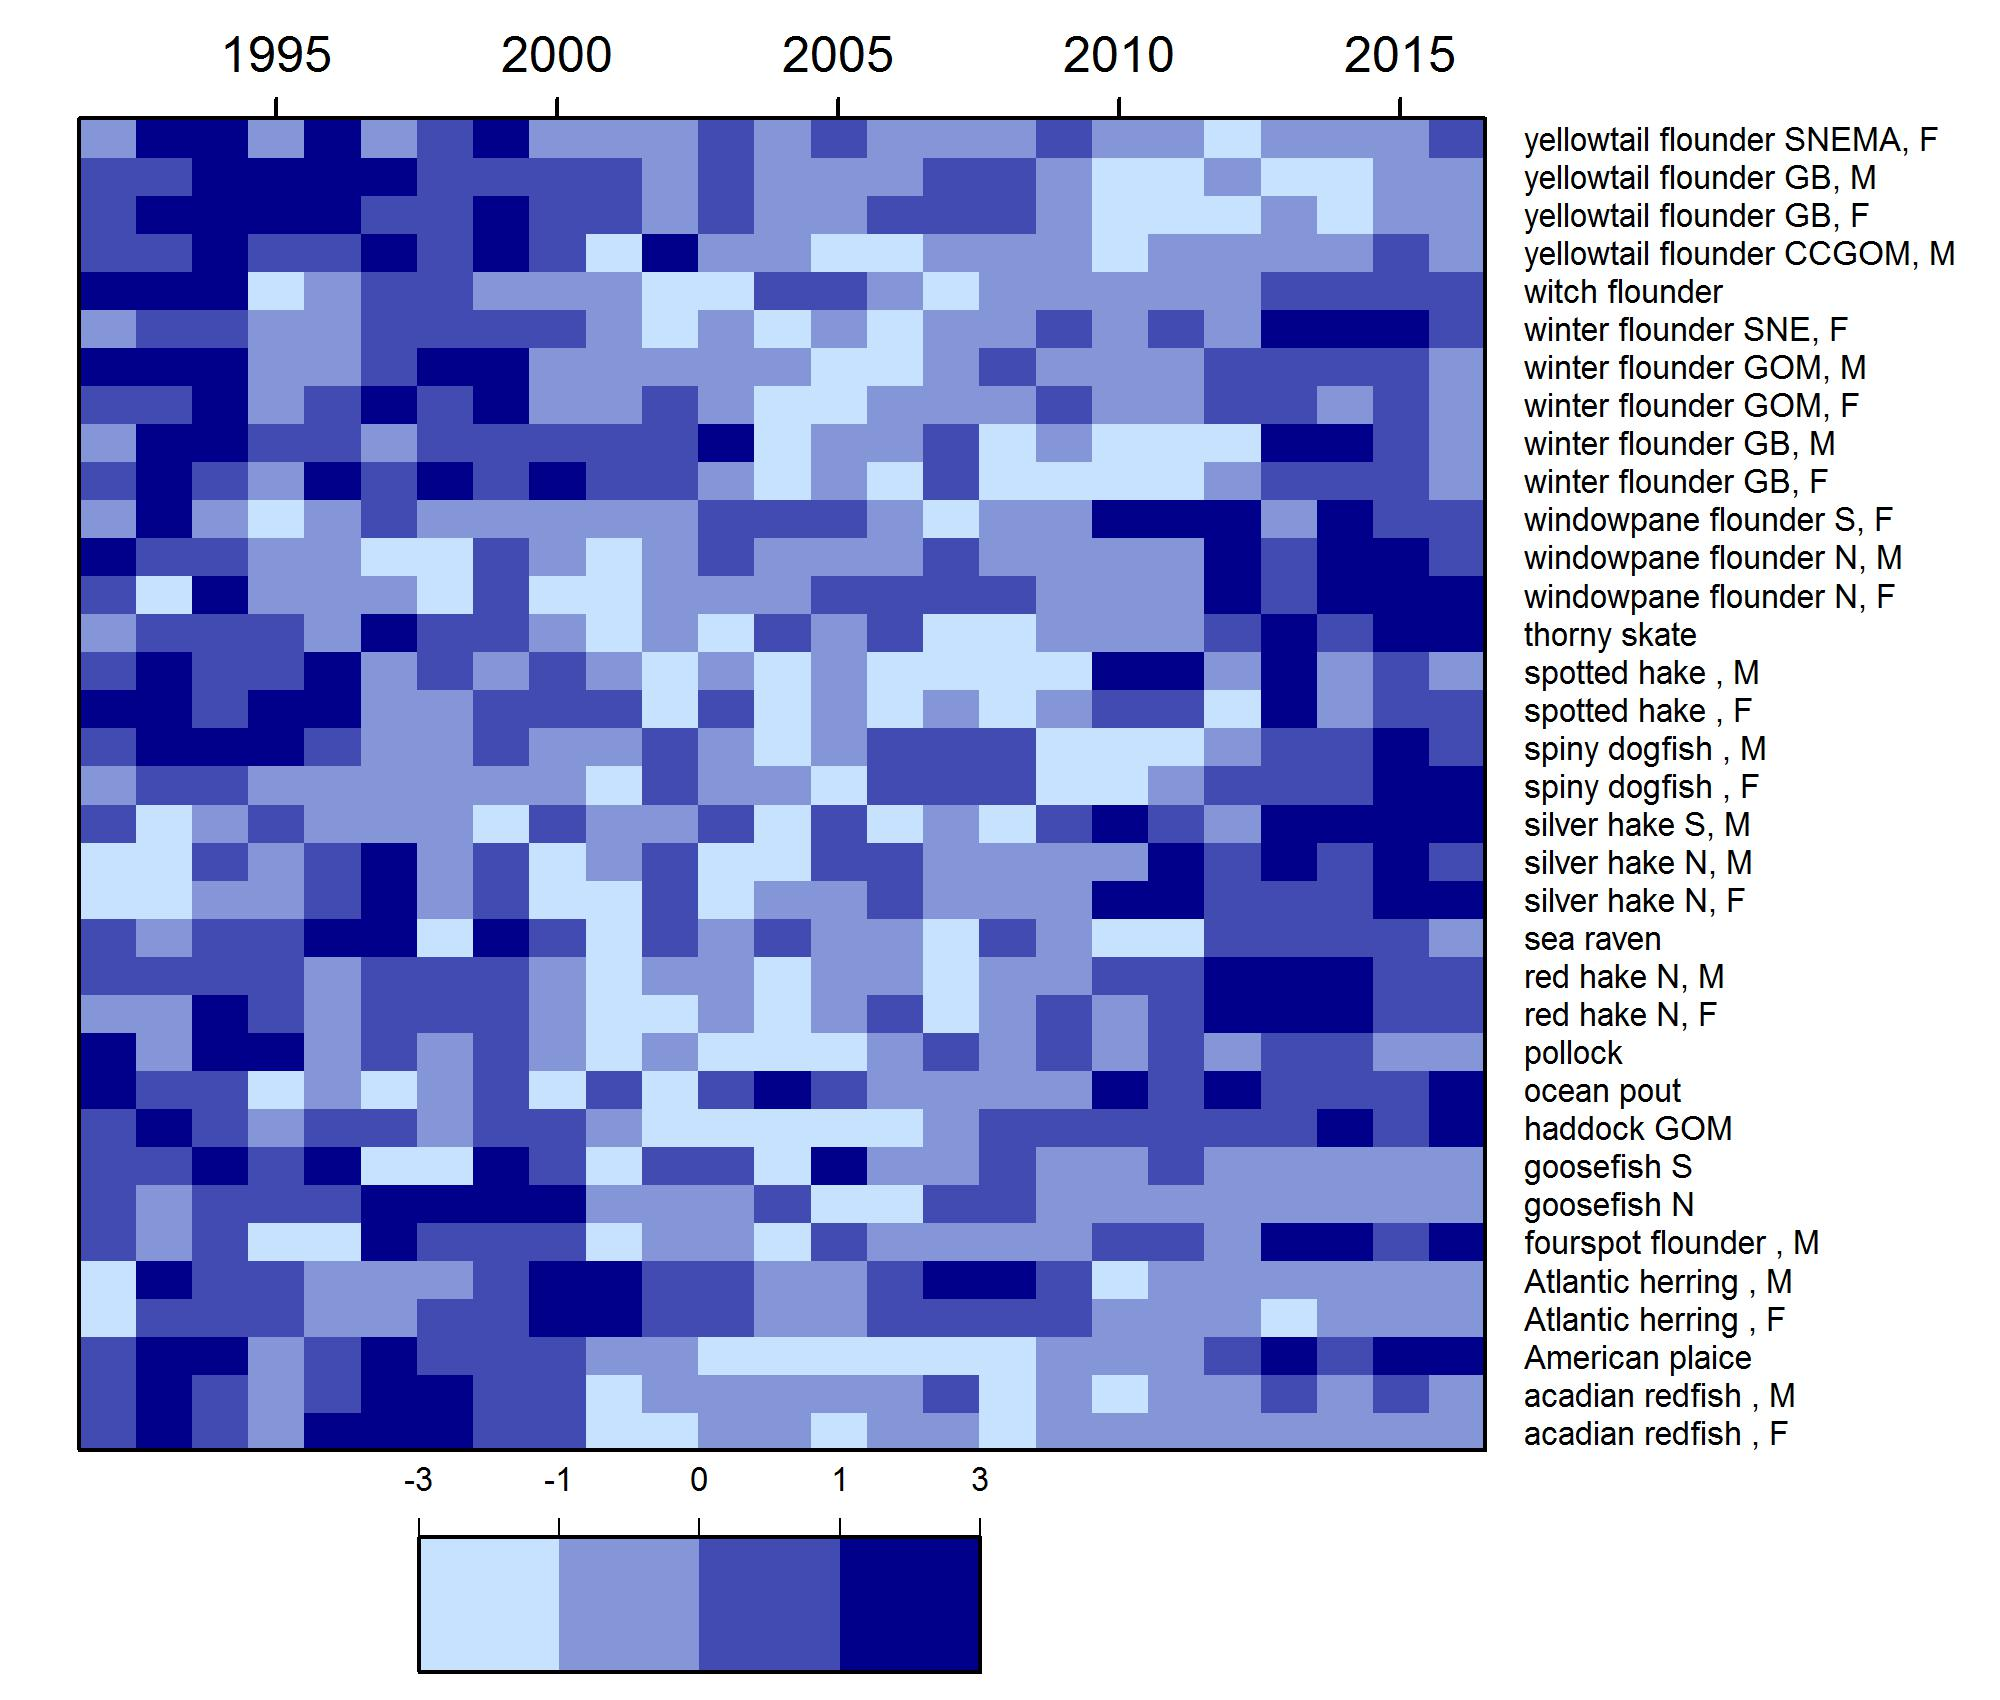
\includegraphics[width=0.7\linewidth]{/users/sgaichas/Documents/0_Data/EBFM_PDT/GBriskassess/RAimages/NEFMC_Fish_Condition} 

}

\caption{Fish Condition (weight/length) \label{cond}}\label{fig:unnamed-chunk-6}
\end{figure}

\subsubsection{Fish productivity}\label{fish-productivity}

The number of small fish relative to the biomass of larger fish of the
same species from the NEFSC survey is a simple measure of productivity,
intended to complement model-based stock assessment estimates of
recruitment for commercial species. There is a no clear trend in this
indicator when aggregated across managed and unmanaged species on
Georges Bank.

\begin{figure}

{\centering 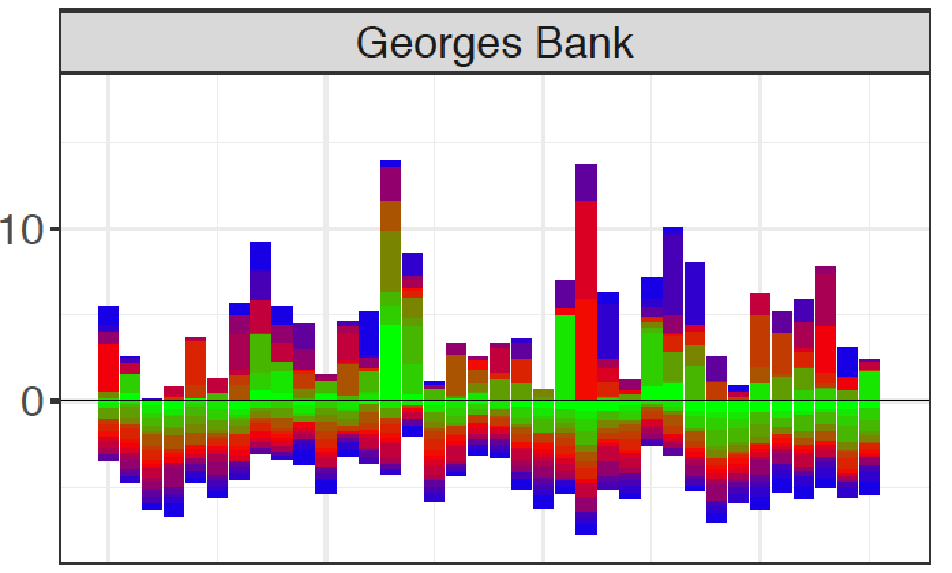
\includegraphics[width=0.7\linewidth]{/users/sgaichas/Documents/0_Data/EBFM_PDT/GBriskassess/RAimages/GBprod} 

}

\caption{Fish productivity: Anomalies of recruit abundance per spawner biomass for species in the MAB. Annual anomalies shown are the average of spring and fall anomalies. \label{fishprodsurvey}}\label{fig:unnamed-chunk-7}
\end{figure}

To summarize, primary production shows no trend. Similarly, there are no
trends in overall zooplankton abundance, but an important New England
species shows a recent decline during fall. Fish condition showed a drop
across all species in the early 2000s, but most species appear to have
recovered. There is no trend in aggregate numbers of small fish per
large fish. The one clear trend in Calanus biovolume (combined with poor
condition for GB yellowtail) suggests a low-moderate risk of changing
ecosystem productivity in the Georges Bank region.

\subsection{Climate}\label{climate}

This element is applied at the species level. Risks to species
productivity (and therefore to achieving OY) due to projected climate
change in the Northeast US were evaluated in a comprehensive assessment
(Hare et al. 2016). This assessment evaluated exposure of each species
to multiple climate threats, including ocean and air temperature, ocean
acidification, ocean salinity, ocean currents, precipitation, and sea
level rise. The assessment also evaluated the sensitivity (\emph{not
extinction risk}) of each species based on habitat and prey specificity,
sensitivity to temperature and ocean acidification, multiple life
history factors, and number of non-climate stressors. This assessment is
intended to be conducted iteratively, so these results can be updated in
the future.

\begin{longtable}[]{@{}ll@{}}
\toprule
Risk Level & Definition\tabularnewline
\midrule
\endhead
Low & Low climate vulnerability ranking\tabularnewline
Low-Moderate & Moderate climate vulnerability ranking\tabularnewline
Moderate-High & High climate vulnerability ranking\tabularnewline
High & Very high climate vulnerability ranking\tabularnewline
\bottomrule
\end{longtable}

New England species were all either highly or very highly exposed to
climate risk in this region, and ranged from low to very high
sensitivity to expected climate change in the Northeast US. The
combination of exposure and sensitivity results in the overall
vulnerability ranking. We applied those climate vulnerability rankings
directly here (Fig. \ref{NEVAvul}).

\begin{figure}

{\centering 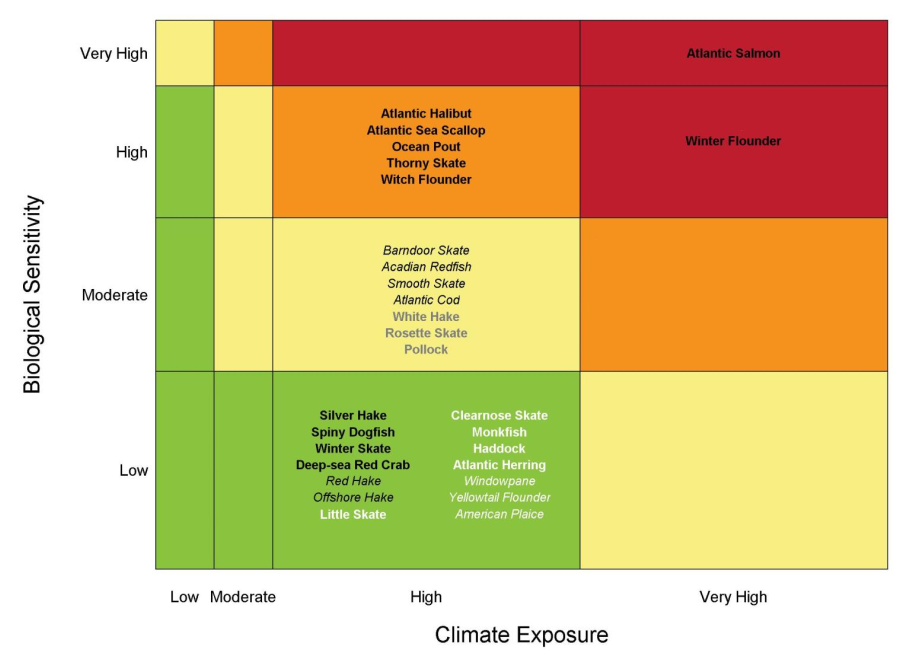
\includegraphics[width=\linewidth]{/users/sgaichas/Documents/0_Data/EBFM_PDT/GBriskassess/RAimages/NEVAvulNE} 

}

\caption{Results of Northeast Climate Vulnerability Analysis (Hare et al. 2016) for Mid-Atlantic species \label{NEVAvul}}\label{fig:unnamed-chunk-9}
\end{figure}

While this risk assessment focuses on overall vulnerability to impacts
of climate, not all impacts will be negative. Some MAFMC managed species
may benefit from projected future climate conditions, including black
sea bass, bluefish, butterfish, longfin squid, and shortfin squid (Hare
et al. 2016). However, all NEFMC managed species were expected to have
either neutral or negative directional effects from expected climate
change (Hare et al. 2016).

\subsection{Distribution Shifts}\label{distribution-shifts}

This element is applied at the species level. Species distribution
shifts can increase risks of ineffective spatial catch allocation; if
catch distribution is greatly mismatched with species distribution OY
may not be achieved. Risks of species distribution shifts due to
projected climate change in the Northeast US were assessed in a
comprehensive assessment (Hare et al. 2016). We applied those
distribution shift risk rankings directly here. In addition, changes in
species distribution are monitored using fisheries independent bottom
trawl surveys. Two distribution shift indicators are derived from these
surveys: kernel density plots of recent distribution compared with 1970s
distribution, and time series of the along shelf position of the center
of distribution.

\begin{longtable}[]{@{}ll@{}}
\toprule
Risk Level & Definition\tabularnewline
\midrule
\endhead
Low & Low potential for distribution shifts\tabularnewline
Low-Moderate & Moderate potential for distribution shifts\tabularnewline
Moderate-High & High potential for distribution shifts\tabularnewline
High & Very high potential for distribution shifts\tabularnewline
\bottomrule
\end{longtable}

Most New England species had either high or very high risk of
distribution shifts in the Northeast US. Sea scallops, ocean pout,
Atlantic salmon, and smooth skate were predicted to have moderate risk
of distribution change (Hare et al. 2016).

\begin{figure}

{\centering 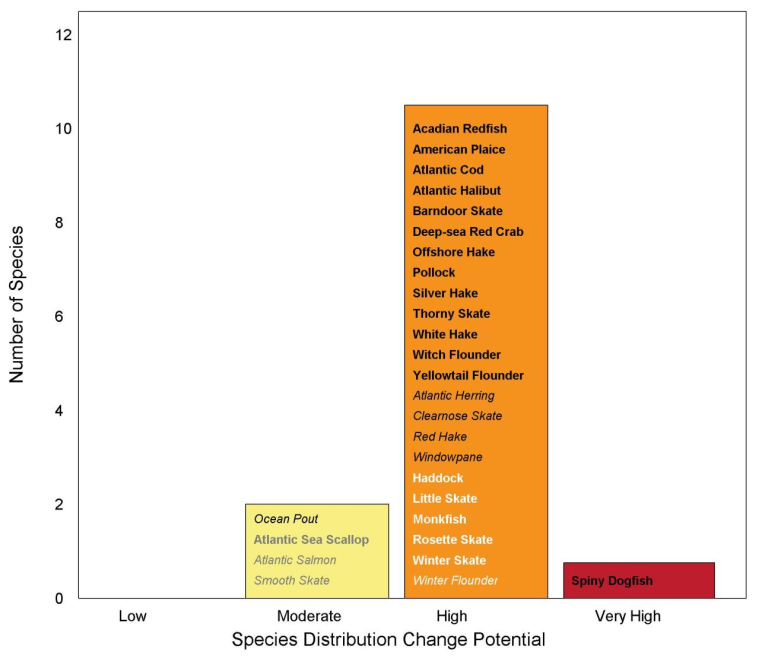
\includegraphics[width=0.8\linewidth]{/users/sgaichas/Documents/0_Data/EBFM_PDT/GBriskassess/RAimages/NEVAshiftNE} 

}

\caption{Results of Northeast Climate Vulnerability Analysis (Hare et al. 2016) for Mid-Atlantic species distribution shift risk \label{NEVAshift}}\label{fig:unnamed-chunk-10}
\end{figure}

\subsubsection{Historical vs.~Current Distribution
Maps}\label{historical-vs.current-distribution-maps}

Spatial distribution has changed over time for some species more than
for others. Yellowtail flounder distributions measured by NEFSC surveys
have shifted northward relative to historical distributions. In
contrast, redfish distributions have remained relatively stable.

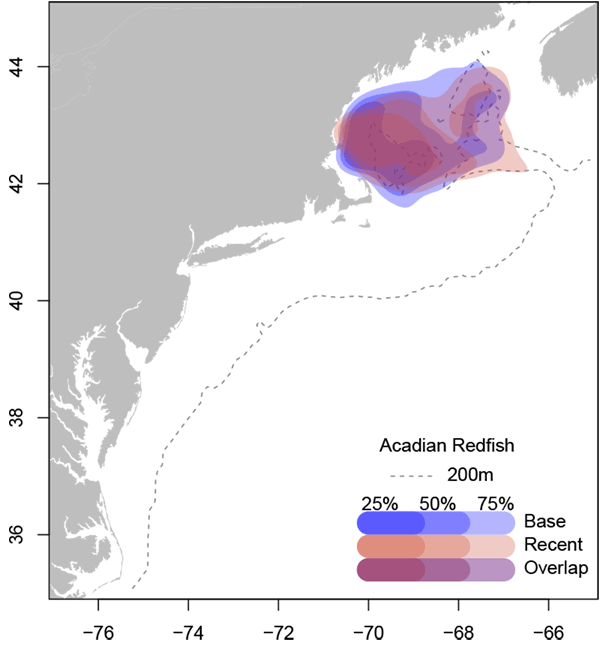
\includegraphics[width=.49\linewidth]{/users/sgaichas/Documents/0_Data/EBFM_PDT/GBriskassess/RAimages/acadian-redfish-kd}
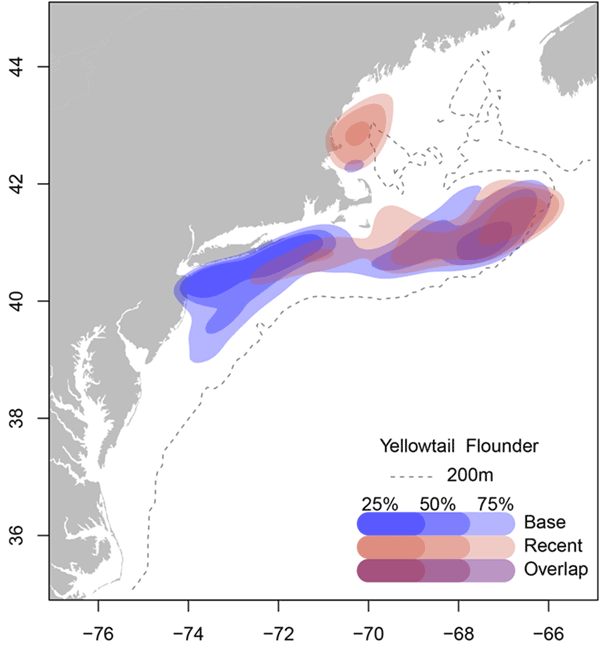
\includegraphics[width=.49\linewidth]{/users/sgaichas/Documents/0_Data/EBFM_PDT/GBriskassess/RAimages/yellowtail-flounder-kd}

\begin{figure}

{\centering \includegraphics{SOE_GB_RiskAssess_files/figure-latex/unnamed-chunk-12-1} 

}

\caption{Shifts in species distribution, 1970s (blue), recent (red) and overlap (purple) \label{dists}}\label{fig:unnamed-chunk-12}
\end{figure}

A full suite of these maps is available at
\url{http://www.nefsc.noaa.gov/ecosys/current-conditions/kernel-density.html}.

\subsubsection{Changes in Along Shelf
Position}\label{changes-in-along-shelf-position}

Species distribution on the NE Shelf can be characterized by the
position in the ecosystem along an axis oriented from the southwest to
the northeast, referred to as the along shelf distance, and by depth.
Along shelf distances range from 0 to 1360, which relates to positions
along the axis from the origin in the southwest to the northeast in
kilometer units. The mean along shelf distance for several NEFMC species
by year is shown below; many are consistent with the predictions of NEVA
and show a significant northeastward change in distribution. Mean depth
has also changed for some of these species. Information for more species
is available at
\url{http://www.nefsc.noaa.gov/ecosys/current-conditions/species-dist.html}.

\begin{figure}

{\centering \includegraphics[width=.49\linewidth]{SOE_GB_RiskAssess_files/figure-latex/unnamed-chunk-13-1} \includegraphics[width=.49\linewidth]{SOE_GB_RiskAssess_files/figure-latex/unnamed-chunk-13-2} 

}

\caption{Shifts in species distribution over time; A: Yellowtail flounder, B: Winter flounder, C: Cod, D: Haddock, E: Atlantic herring, F: Acadian redfish \label{shifts}}\label{fig:unnamed-chunk-13}
\end{figure}

\subsection{Estuarine and Coastal
Habitat}\label{estuarine-and-coastal-habitat}

This element is applied at the species level. Risk of not achieving OY
due to threats to estuarine and nearshore coastal habitat/nursery
grounds was determined by first evaluating the estuarine dependence of
species, and then by enumerating threats to the estuarine habitat
required by these species. Here, we include estuarine and nearshore
coastal habitat in the term ``estuarine'' below. Water and habitat
quality assessments produced for coastal estuaries within the Northeast
region can be considered in the future.

\begin{longtable}[]{@{}ll@{}}
\toprule
Risk Level & Definition\tabularnewline
\midrule
\endhead
Low & Not dependent on nearshore coastal or estuarine
habitat\tabularnewline
Low-Moderate & Estuarine dependent, estuarine condition
stable\tabularnewline
Moderate-High & Estuarine dependent, estuarine condition
fair\tabularnewline
High & Estuarine dependent, estuarine condition poor\tabularnewline
\bottomrule
\end{longtable}

As a start, the US EPA National Coastal Condition Assessment for the
Northeast US (US EPA 2012) was used to evaluate estuarine and coastal
condition. This report lists water, sediment, benthic, and coastal
habitat quality as well as fish contamination. Northeast US coastal
waters rated fair to poor for water quality, fair for sediment quality,
poor for benthic quality, good to fair for coastal habitat, and fair to
poor for fish contamination. These ratings were based on nearshore and
estuarine summer sampling 2003-2006. The overall coastal condition was
rated fair for the entire region, but this includes offshore conditions
which we address in the next element. Therefore, estuarine and nearshore
coastal habitat dependent species (winter flounder (obligate), pollock
(obligate?), and white and red hake (facultative), (Able 2005)) were
ranked high risk based on overall poor estuarine condition for this
element, and all others were ranked low risk due to lower dependence on
this habitat type.

\subsection{\texorpdfstring{Offshore Habitat \emph{need access to model
output for NE species if
ranking}}{Offshore Habitat need access to model output for NE species if ranking}}\label{offshore-habitat-need-access-to-model-output-for-ne-species-if-ranking}

This element is applied at the species level. The risk of achieving OY
due to changes in offshore habitat quality and quantity can be assessed
using trends derived from experimental species-specific habitat
modeling. \emph{In addition, the number of threats from other human uses
can be enumerated; at present this is addressed under ``Other Ocean
Uses'' in the Management section below.}

\begin{longtable}[]{@{}ll@{}}
\toprule
\begin{minipage}[b]{0.22\columnwidth}\raggedright\strut
Risk Level\strut
\end{minipage} & \begin{minipage}[b]{0.72\columnwidth}\raggedright\strut
Definition\strut
\end{minipage}\tabularnewline
\midrule
\endhead
\begin{minipage}[t]{0.22\columnwidth}\raggedright\strut
Low\strut
\end{minipage} & \begin{minipage}[t]{0.72\columnwidth}\raggedright\strut
No change in offshore habitat quality or quantity\strut
\end{minipage}\tabularnewline
\begin{minipage}[t]{0.22\columnwidth}\raggedright\strut
Low-Moderate\strut
\end{minipage} & \begin{minipage}[t]{0.72\columnwidth}\raggedright\strut
Increasing variability in habitat quality or quantity\strut
\end{minipage}\tabularnewline
\begin{minipage}[t]{0.22\columnwidth}\raggedright\strut
Moderate-High\strut
\end{minipage} & \begin{minipage}[t]{0.72\columnwidth}\raggedright\strut
Significant long term decrease in habitat quality or quantity\strut
\end{minipage}\tabularnewline
\begin{minipage}[t]{0.22\columnwidth}\raggedright\strut
High\strut
\end{minipage} & \begin{minipage}[t]{0.72\columnwidth}\raggedright\strut
Significant recent decrease in habitat quality or quantity\strut
\end{minipage}\tabularnewline
\bottomrule
\end{longtable}

Habitat models using both static and dynamics variables have been
developed for many of the resource species on the Northeast Shelf. These
models estimate spring and fall habitat for the time series 1992 to 2016
reflecting the use of the ecosystem based on the NEFSC bottom trawl
survey. The variables evaluated for use in these models included station
salinity, station temperature, benthic complexity, satellite derived
chlorophyll concentration and sea surface temperature, the gradient
magnitude (front structure) of the satellite data, and zooplankton
bio-volume and taxa abundance with station depth included in all models.
The random forest approach differentiates variables with strong
predictive power and was used to reduce the variable set to 11 variables
for each species. The models were used to estimate fall habitat scores
over the entire shelf over the time series.

\begin{figure}

{\centering \includegraphics{SOE_GB_RiskAssess_files/figure-latex/unnamed-chunk-14-1} 

}

\caption{Shifts in modeled species fall habitat area over time; A: Black sea bass, B: Summer flounder, C: Scup, D: Butterfish, E: Atlantic mackerel, F: Longfin squid, G: Shortfin squid, H: Dogfish, I: Goosefish  \label{shifts}}\label{fig:unnamed-chunk-14}
\end{figure}

\emph{This experimental habitat index is still being studied and
improved, so habitat risk rankings based on this are considered
preliminary by the EOP.}

Overall, black sea bass, summer flounder, and scup have long term
increasing trends in fall offshore habitat, and dogfish, butterfish,
Atlantic mackerel and longfin squid have short term increasing trends.
Goosefish has no significant trend in fall offshore habitat. Therefore,
these species rank low risk for this element. However, shortfin squid
has a long term and a short term decreasing trend in offshore habitat.
Therefore, shortfin squid ranks high risk for this element.

Ocean quahogs, surfclams, tilefish, and bluefish are not adequately
sampled by the bottom trawl survey and were not included in this
analysis, similar to unmanaged forage and deepsea corals. Sessile
species in particular may be highly vulnerable to habitat changes, so
assessments of their habitat are particularly important to develop.

\section{Economic Elements}\label{economic-elements}

\subsection{Commercial Revenue}\label{commercial-revenue}

This element is applied at the ecosystem level, and addresses the risk
of not maximizing fishery value. Revenue serves as a proxy for
commercial profits, which is the component of a fishery's value that
this element is ultimately attempting to assess risk towards.

\begin{longtable}[]{@{}ll@{}}
\toprule
Risk Level & Definition\tabularnewline
\midrule
\endhead
Low & No trend and low variability in revenue\tabularnewline
Low-Moderate & Increasing or high variability in revenue\tabularnewline
Moderate-High & Significant long term revenue decrease\tabularnewline
High & Significant recent decrease in revenue\tabularnewline
\bottomrule
\end{longtable}

This is aggregate commercial revenue for NEFMC managed species. There is
a long term significant decrease in revenue for GB, indicating
moderate-high risk to commercial fishery profit. This trend is
consistent with the trend first shown in the EAFM Interactions white
paper and published in Gaichas et al. (2016) (Figs 2-3).

\begin{figure}

{\centering \includegraphics{SOE_GB_RiskAssess_files/figure-latex/ComProfAgg-1} 

}

\caption{Aggregate New England managed species revenue  \label{comprofagg}}\label{fig:ComProfAgg}
\end{figure}

\subsection{Marine Recreational Angler
Days/Trips}\label{marine-recreational-angler-daystrips}

This element is applied at both the fleet level and at the ecosystem
level where it would apply equally to all recreationally fished species.
Angler days and trips are proxies for the welfare (value) generated from
recreational fishing. Risk of not maximizing fishery value is evaluated
using the number of marine recreational fishing angler-days and number
of marine recreational trips, in aggregate.

\begin{longtable}[]{@{}ll@{}}
\toprule
Risk Level & Definition\tabularnewline
\midrule
\endhead
Low & No trends in angler days/trips\tabularnewline
Low-Moderate & Increasing or high variability in angler
days/trips\tabularnewline
Moderate-High & Significant long term decreases in angler
days/trips\tabularnewline
High & Significant recent decreases in angler days/trips\tabularnewline
\bottomrule
\end{longtable}

Providing recreational opportunities is a stated goal of optimal fishery
management as part of the definition of ``benefits to the nation'' under
MSA. Recreational fishing is important in the Northeast region with many
coastal communities having high recreational dependence. Although there
is an overall trend of increasing recreational fishery participation in
terms of number of anglers, the most recent 10 years has shown a
striking decline in both recreation indices.

\begin{figure}

{\centering \includegraphics{SOE_GB_RiskAssess_files/figure-latex/Rec Participation-1} 

}

\caption{A: number of anglers, B: number of trips \label{recreation}}\label{fig:Rec Participation}
\end{figure}

These significant recent decreases in numbers of anglers and numbers of
trips alone suggest high risk to recreational value generated from the
species with substantial recreational fisheries. This is a national
trend likely due to shifting demographics and general economic dynamics,
among other issues.

\subsection{Commercial Fishery Resilience (Revenue
Diversity)}\label{commercial-fishery-resilience-revenue-diversity}

This element is applied at the ecosystem level. This element addresses
the risk of reduced commercial fishery business resilience by evaluating
species diversity of revenue at the permit level.

\begin{longtable}[]{@{}ll@{}}
\toprule
Risk Level & Definition\tabularnewline
\midrule
\endhead
Low & No trend in diversity measure\tabularnewline
Low-Moderate & Increasing or high variability in diversity
measure\tabularnewline
Moderate-High & Significant long term downward trend in diversity
measure\tabularnewline
High & Significant recent downward trend in diversity
measure\tabularnewline
\bottomrule
\end{longtable}

This diversity index is the average effective Shannon index for species
revenue at the permit level, for all permits landing any amount of NEFMC
FMP species within a year (including both Monkfish and Spiny Dogfish).
Although the exact value of the effective Shannon index is relatively
uninformative, the major change in diversity seems to have occurred in
the late 1990's, with much of the recent index relatively stable.

\begin{figure}

{\centering \includegraphics{SOE_GB_RiskAssess_files/figure-latex/unnamed-chunk-15-1} 

}

\caption{Diversity in species revenue \label{fleetsppdiv}}\label{fig:unnamed-chunk-15}
\end{figure}

This index shows no significant trend, which would suggest a low risk to
fishery business resilience based on diversity in species revenue.

\subsection{\texorpdfstring{Commercial Fishery Resilience (Shoreside
Support) \emph{need access to state data for New England if
ranking}}{Commercial Fishery Resilience (Shoreside Support) need access to state data for New England if ranking}}\label{commercial-fishery-resilience-shoreside-support-need-access-to-state-data-for-new-england-if-ranking}

This element is applied at the ecosystem level. This element ranks the
risk of reduced fishery business resilience due to shoreside support
infrastructure by examining the number of shoreside support businesses.

\begin{longtable}[]{@{}ll@{}}
\toprule
\begin{minipage}[b]{0.22\columnwidth}\raggedright\strut
Risk Level\strut
\end{minipage} & \begin{minipage}[b]{0.72\columnwidth}\raggedright\strut
Definition\strut
\end{minipage}\tabularnewline
\midrule
\endhead
\begin{minipage}[t]{0.22\columnwidth}\raggedright\strut
Low\strut
\end{minipage} & \begin{minipage}[t]{0.72\columnwidth}\raggedright\strut
No trend in shoreside support businesses\strut
\end{minipage}\tabularnewline
\begin{minipage}[t]{0.22\columnwidth}\raggedright\strut
Low-Moderate\strut
\end{minipage} & \begin{minipage}[t]{0.72\columnwidth}\raggedright\strut
Increasing or high variability in shoreside support businesses\strut
\end{minipage}\tabularnewline
\begin{minipage}[t]{0.22\columnwidth}\raggedright\strut
Moderate-High\strut
\end{minipage} & \begin{minipage}[t]{0.72\columnwidth}\raggedright\strut
Significant recent decrease in one measure of shoreside support
businesses\strut
\end{minipage}\tabularnewline
\begin{minipage}[t]{0.22\columnwidth}\raggedright\strut
High\strut
\end{minipage} & \begin{minipage}[t]{0.72\columnwidth}\raggedright\strut
Significant recent decrease in multiple measures of shoreside support
businesses\strut
\end{minipage}\tabularnewline
\bottomrule
\end{longtable}

The number of shoreside support businesses were tallied for all
Mid-Atlantic states in two categories: number of companies (Quarterly
Census of Employment and Wages. Obtained September 27, 2017. US
Department of Labor, Bureau of Labor Statistics.
\url{https://www.bls.gov/cew/home.htm}) and number of non-employer
entities Nonemployer Statistics.'' Obtained September 28, 2017. U.S.
Census Bureau.
\url{https://www.census.gov/programs-surveys/nonemployer-statistics.html}),
which we consider separately. Nonemployer entities are businesses that
have no paid employees (i.e.~the owner is the workforce), while the
shoreside support companies include all businesses with paid employees.
Some state level data was not included due to confidentiality.

\begin{figure}

{\centering \includegraphics{SOE_GB_RiskAssess_files/figure-latex/Shoresupp1-1} 

}

\caption{Shoreside support businesses: Number of Companies  \label{shoresupp1}}\label{fig:Shoresupp1}
\end{figure}

\begin{figure}

{\centering \includegraphics{SOE_GB_RiskAssess_files/figure-latex/Shoresupp2-1} 

}

\caption{Shoreside support businesses: Number of Nonemployer entities  \label{shoresupp2}}\label{fig:Shoresupp2}
\end{figure}

The number of shoreside support companies that include seafood merchant
wholesalers, seafood product preparation and packaging, and seafood
markets across all Mid-Atlantic states shows a significant long term and
short term decrease, which on its own represents moderate-high risk to
fishery resilience. However, the number of non-employer entities which
include seafood preparation and packaging and seafood markets shows a
long term increase. Trends in other shoreside fishery supporting
businesses such as gear manufacturers and welding companies are not
included here due to aggregation of the statistics.

\subsection{\texorpdfstring{Commercial Employment \emph{need state level
data for NE if
ranking}}{Commercial Employment need state level data for NE if ranking}}\label{commercial-employment-need-state-level-data-for-ne-if-ranking}

This element is applied at the state level. This element ranks the risk
of not optimizing employment opportunities in the commercial sector.
Risks were assessed by examining time series of employment information
from Fisheries Economics of the U.S. (NMFS 2017). A full description of
the model generating employment estimates can be found here:
\url{http://www.st.nmfs.noaa.gov/documents/commercial_seafood_impacts_2007-2009.pdf}

\begin{longtable}[]{@{}ll@{}}
\toprule
Risk Level & Definition\tabularnewline
\midrule
\endhead
Low & No trend in employment\tabularnewline
Low-Moderate & Increasing or high variability in
employment\tabularnewline
Moderate-High & Significant recent decrease in employment for one
state\tabularnewline
High & Significant recent decrease in employment for multiple
states\tabularnewline
\bottomrule
\end{longtable}

The EOP Committee lacked confidence in the available employment
indicator data, so this element remains unranked at this time.

\subsection{\texorpdfstring{Recreational Employment \emph{need state
level data for NE if
ranking}}{Recreational Employment need state level data for NE if ranking}}\label{recreational-employment-need-state-level-data-for-ne-if-ranking}

This element is applied at the state level. This element ranks the risk
of not optimizing employment opportunities in the recreational sector.
Risks were assessed by examining time series of employment information
from Fisheries Economics of the U.S. (NMFS 2017).

\begin{longtable}[]{@{}ll@{}}
\toprule
Risk Level & Definition\tabularnewline
\midrule
\endhead
Low & No trend in employment\tabularnewline
Low-Moderate & Increasing or high variability in
employment\tabularnewline
Moderate-High & Significant recent decrease in employment for one
state\tabularnewline
High & Significant recent decrease in employment for multiple
states\tabularnewline
\bottomrule
\end{longtable}

The EOP Committee lacked confidence in the available employment
indicator data, so this element remains unranked at this time.

\section{Social-Cultural Elements}\label{social-cultural-elements}

\subsection{Fleet Diversity}\label{fleet-diversity}

This element is applied at the ecosystem level. This element ranks the
risk to maintaining equity in access to fishery resources. Two
indicators of commercial fleet diversity, including the number of
distinct fleets and diversity of revenue across fleets are used in
combination to evaluate current fleet resilience throughout the New
England region.

Maintaining diversity can provide the capacity to adapt to change at the
ecosystem level for dependent fishing communities, and can address
objectives related to stability. Below are diversity estimates for
fleets landing NEFMC-managed species. This measure identifies the
diversity in revenue generated by different fleet segments. A fleet is
defined here as the combination of gear code (Scallop Dredge, Other
Dredge, Gillnet, Hand Gear, Longline, Bottom Trawl, Midwater Trawl, Pot,
Purse Seine, or Clam Dredge) and vessel length category (Less than 30
ft, 30 to 50 ft, 50 to 75 feet, 75 ft and above).

\begin{longtable}[]{@{}ll@{}}
\toprule
Risk Level & Definition\tabularnewline
\midrule
\endhead
Low & No trend in diversity measure\tabularnewline
Low-Moderate & Increasing or high variability in diversity
measure\tabularnewline
Moderate-High & Significant long term downward trend in diversity
measure\tabularnewline
High & Significant recent downward trend in diversity
measure\tabularnewline
\bottomrule
\end{longtable}

A declining trend in diversity indicates a less diverse fleet is
currently active in NEFMC-managed fisheries. However, it cannot
distinguish whether specialization (by choice), or alternatively
stovepiping (constrained choices), is occurring in the Northeastern
Large Marine Ecosystem, rather merely that the fleet composition is
changing, which might warrant additional scrutiny.

\begin{figure}

{\centering \includegraphics{SOE_GB_RiskAssess_files/figure-latex/Fleet Diversity-1} 

}

\caption{A: fleet count, B: average fleet diversity  \label{fleetdiv}}\label{fig:Fleet Diversity}
\end{figure}

There is a long term decrease in the fleet count metric. Therefore this
element ranks moderate-high risk.

\subsection{Community Vulnerability}\label{community-vulnerability}

The NOAA Fisheries Community Social Vulnerability Indicators (CSVIs;
Jepson and Colburn (2013)) are statistical measures of the vulnerability
of communities to events such as regulatory changes to fisheries, wind
farms, and other ocean-based businesses, as well as to natural hazards,
disasters, and climate change. The CSVIs currently serve as indicators
of social vulnerability, gentrification pressure vulnerability,
commercial and recreational fishing dependence (with dependence being a
function of both reliance and engagement), sea level rise risk, species
vulnerability to climate change, and catch composition diversity. We use
a combination of these five indicators for the most fishery dependent
communities to evaluate overall social risk levels.

\begin{longtable}[]{@{}ll@{}}
\toprule
\begin{minipage}[b]{0.22\columnwidth}\raggedright\strut
Risk Level\strut
\end{minipage} & \begin{minipage}[b]{0.72\columnwidth}\raggedright\strut
Definition\strut
\end{minipage}\tabularnewline
\midrule
\endhead
\begin{minipage}[t]{0.22\columnwidth}\raggedright\strut
Low\strut
\end{minipage} & \begin{minipage}[t]{0.72\columnwidth}\raggedright\strut
Few (\textless{}10\%) vulnerable fishery dependent communities\strut
\end{minipage}\tabularnewline
\begin{minipage}[t]{0.22\columnwidth}\raggedright\strut
Low-Moderate\strut
\end{minipage} & \begin{minipage}[t]{0.72\columnwidth}\raggedright\strut
10-25\% of fishery dependent communities with \textgreater{}3 high
vulnerability ratings\strut
\end{minipage}\tabularnewline
\begin{minipage}[t]{0.22\columnwidth}\raggedright\strut
Moderate-High\strut
\end{minipage} & \begin{minipage}[t]{0.72\columnwidth}\raggedright\strut
25-50\% of fishery dependent communities with \textgreater{}3 high
vulnerability ratings\strut
\end{minipage}\tabularnewline
\begin{minipage}[t]{0.22\columnwidth}\raggedright\strut
High\strut
\end{minipage} & \begin{minipage}[t]{0.72\columnwidth}\raggedright\strut
Majority (\textgreater{}50\%) of fishery dependent communities with
\textgreater{}3 high vulnerability ratings\strut
\end{minipage}\tabularnewline
\bottomrule
\end{longtable}

Below is a brief description for each category based on the NOAA social
indicator study (Jepson and Colburn 2013, Colburn et al. 2016):

\begin{itemize}
\tightlist
\item
  \textbf{Fishing dependence} indices portray the importance or level of
  dependence of commercial or recreational fishing to coastal
  communities.
\item
  \textbf{Social vulnerability} indices represent social factors that
  can shape either an individual or community's ability to adapt to
  change. These factors exist within all communities regardless of the
  importance of fishing.
\item
  \textbf{Gentrification pressure} indices characterize those factors
  that, over time may indicate a threat to commercial or recreational
  working waterfront, including infrastructure.
\end{itemize}

Communities are ranked as high, medium high, moderate, or low relative
to the respective indicator (Table \ref{reliance}). Community dependence
on commercial and recreational fishing is mixed, with notably more
communities in the Mid-Atlantic dependent on recreational fishing than
in New England.

\begin{table}[h] \centering  
\begin{tabular}{lrrrr}
\toprule
  & Low & Moderate & MedHigh & High\\
\midrule
ME & 109 & 20 & 9 & 34\\
NH & 34 & 5 & 0 & 1\\
MA & 124 & 21 & 4 & 4\\
RI & 33 & 3 & 0 & 2\\
CT & 72 & 3 & 0 & 0\\
\addlinespace
NY & 336 & 7 & 2 & 2\\
NJ & 297 & 11 & 3 & 3\\
PA & 40 & 1 & 0 & 0\\
DE & 69 & 2 & 1 & 2\\
MD & 239 & 4 & 0 & 2\\
\addlinespace
VA & 99 & 3 & 2 & 1\\
NC & 113 & 6 & 3 & 4\\
\bottomrule
\end{tabular} \hspace{1cm} \centering  
\begin{tabular}{lrrrr}
\toprule
  & Low & Moderate & MedHigh & High\\
\midrule
ME & 159 & 11 & 1 & 1\\
NH & 36 & 3 & 1 & 0\\
MA & 129 & 10 & 7 & 7\\
RI & 33 & 5 & 0 & 0\\
CT & 69 & 5 & 1 & 0\\
\addlinespace
NY & 311 & 24 & 6 & 6\\
NJ & 283 & 18 & 8 & 5\\
PA & 41 & 0 & 0 & 0\\
DE & 62 & 3 & 1 & 8\\
MD & 218 & 14 & 6 & 7\\
\addlinespace
VA & 89 & 10 & 3 & 3\\
NC & 85 & 13 & 8 & 20\\
\bottomrule
\end{tabular} \caption{Number of communities at each level of commercial (left) and recreational (right) reliance\label{reliance}} \end{table}

The social and economic impacts of climate change have been modeled
through application of social indicators of fishing dependent
communities (Jepson and Colburn 2013). Assessment of a range of social
indicators has been applied in the Mid-Atlantic Region to predict
vulnerability of communities to regulatory changes and disasters. More
recently this methodology has been extended to include specific
indicators of vulnerability to climate change and linked to species
vulnerability assessments (Colburn et al. 2016, Hare et al. 2016). The
tools developed through this approach are vital to an evaluation of the
risks of climate change facing coastal communities dependent on fishing.
Below is a description of the CSVIs related to climate change.

\begin{itemize}
\tightlist
\item
  \textbf{Sea Level Rise Index} is a measure of the overall risk of
  inundation from sea level rise based on community area lost from one
  to six foot level projections over the next \textasciitilde{}90 years.
  A high rank indicates a community more vulnerable to sea level rise.
\item
  \textbf{Species Vulnerability} is measured by the proportion of
  community fish landings that attributed to species vulnerable to
  climate change.
\item
  \textbf{Catch Composition Diversity} is the relative abundance of
  species landed in a community. It is measured by Simpson's Reciprocal
  Index, and a higher index value indicates greater diversity.
  Communities with a diverse array of species landed may be less
  vulnerable to climate change.
\end{itemize}

Sea level rise is predicted to have variable impacts on coastal
communities. The Mid-Atlantic region has a 3-4 times higher than global
average sea level rise rate (Sallenger et al. 2012). Mid-Atlantic
communities clustered around the Chesapeake Bay area and the New Jersey
shore had especially high vulnerability to sea level rise (Fig.
\ref{commrisk}). These vulnerabilities include infrastructure (docks,
marinas, bait shops, gear storage) and access to shore-based facilities
due realignment of coastal communities.

Mid-Atlantic fishing communities with total landings value of \$100,000
or more were mapped for their dependence on species vulnerable to
climate change and catch composition diversity (Simpson Reciprocal
Index). A number of communities in southern New Jersey, Maryland and
Virginia are highly dependent on species such as clams that are highly
vulnerable to climate change while displaying low catch composition
diversity. Communities with this situation are considered more
vulnerable to climate change in general.

Assessment of the potential impacts of climate change on recreational
and commercial fishermen and their communities has begun by linking
social and economic indicators of community vulnerability and resilience
to the climate vulnerability assessments of biological and ecological
change expected to result from climate change and sea-level rise.
Fishing communities in New England have generally moderate to low risks
from sea level rise compared with communities in the Mid-Atlantic.
However, there is moderate to high reliance on species vulnerable to
climate in New England, and generally low catch diversity for
communities in the Gulf of Maine, which may also increase risk.

\begin{figure}

{\centering \includegraphics{SOE_GB_RiskAssess_files/figure-latex/Community Risk NE-1} 

}

\caption{Risks from sea level rise (A), reliance on climate-vulnerable species (B), and catch diversity (C) \label{commrisk}}\label{fig:Community Risk NE}
\end{figure}

While the maps provides an overview of the social and climate indicator
results for the New England coastal communities, Table \ref{community}
identifies Mid-Atlantic communities that are most highly dependent on
both commercial and recreational fishing. \emph{This analysis would need
to be redone for New England communities if the New England Council
wishes to use this element.} The varying vulnerability level to social
factors, gentrification pressure, and climate change in these
communities provide a more comprehensive profile and should be taken
into account in the decision making process for fishery management.

As a preliminary risk assessment, rankings from Table \ref{community} of
MedHigh or High were tallied for social vulnerability and gentrification
pressure, along with rankings of High risk from sea level rise,
High/Very High species vulnerability, and rankings of Low catch
composition diversity. Four of these communities (20\%) have three or
more of these high risk rankings, so we rank overall social-cultural
risk as low-moderate for these Mid-Atlantic communities.

\begin{table}

\caption{\label{tab:communitytab}Selected Mid-Atlantic Fishing Communities with Medium High to High Dependence on both Commercial and Recreational Fishing \label{community}}
\centering
\resizebox{\linewidth}{!}{\begin{tabular}[t]{l>{\raggedright\arraybackslash}p{7em}>{\raggedright\arraybackslash}p{7em}>{\raggedright\arraybackslash}p{7em}>{\raggedright\arraybackslash}p{7em}>{\raggedright\arraybackslash}p{7em}>{\raggedright\arraybackslash}p{7em}>{\raggedright\arraybackslash}p{7em}}
\toprule
Community & Commercial Fishing Dependence & Recreational Fishing Dependence & Social Vulnerability & Gentrification Pressure & Sea Level Rise Risk & Species Vulnerability & Catch Composition Diversity\\
\midrule
Hampton Bays, NY & High & High & Low & MedHigh & Medium & Mixed & Moderate\\
Montauk, NY & High & High & Medium & MedHigh & Medium & Mixed & High\\
Barnegat Light, NJ & High & High & Medium & High & Low & High/Very High & Low\\
Cape May, NJ & High & High & Medium & MedHigh & Medium & High/Very High & Low\\
Beaufort, NC & High & High & MedHigh & Low & Low & Mixed & Low\\
\addlinespace
Wanchese, NC & High & High & Medium & Low & Medium & Mixed & High\\
Point Lookout, NY & MedHigh & High & Low & MedHigh & Low & High/Very High & Low\\
Belmar, NJ & MedHigh & High & Medium & Medium & Low & Moderate & Low\\
Point Pleasant, NJ & MedHigh & High & Low & Medium & Medium & High/Very High & Moderate\\
Waretown, NJ & MedHigh & High & Low & Medium & Low & Low & Low\\
\addlinespace
Ocean City, MD & MedHigh & High & Medium & Medium & Medium & Mixed & High\\
Aurora, NC & MedHigh & High & MedHigh & Medium & Low & N/A & N/A\\
Hatteras, NC & MedHigh & High & Medium & Low & N/A & Mixed & High\\
Oriental, NC & MedHigh & High & Medium & Medium & Low & Mixed & Low\\
Chincoteague, VA & MedHigh & High & Medium & Medium & High & Moderate & Moderate\\
\addlinespace
Wachapreague, VA & MedHigh & High & Medium & Medium & Low & High/Very High & Moderate\\
Sea Isle City, NJ & MedHigh & MedHigh & Medium & MedHigh & Medium & Moderate & Low\\
Bowers, DE & MedHigh & MedHigh & Medium & Medium & Low & N/A & N/A\\
Hobucken, NC & MedHigh & MedHigh & Medium & Medium & N/A & Mixed & Low\\
Swan Quarter, NC & MedHigh & MedHigh & MedHigh & Low & N/A & Mixed & Low\\
\addlinespace
Hampton, VA & MedHigh & MedHigh & MedHigh & Low & High & Moderate & Moderate\\
Newport News, VA & MedHigh & MedHigh & MedHigh & Low & High & High/Very High & Low\\
\bottomrule
\end{tabular}}
\end{table}

More information on Northeast coastal communities is available here:
\url{http://www.nefsc.noaa.gov/read/socialsci/communityProfiles.html}

\clearpage

\section{Food Production Elements}\label{food-production-elements}

\subsection{Commercial Seafood
Provision}\label{commercial-seafood-provision}

This element is applied at the ecosystem level. This element describes
the risk of not optimizing domestic seafood production from MAFMC
managed species. Commercial seafood landings (as opposed to total
landings which include bait and industrial uses) were used to assess
seafood provision.

\begin{longtable}[]{@{}ll@{}}
\toprule
Risk Level & Definition\tabularnewline
\midrule
\endhead
Low & No trend or increase in seafood landings\tabularnewline
Low-Moderate & Increasing or high variability in seafood
landings\tabularnewline
Moderate-High & Significant long term decrease in seafood
landings\tabularnewline
High & Significant recent decrease in seafood landings\tabularnewline
\bottomrule
\end{longtable}

Total commercial seafood landings from all species and from NEFMC
managed species indicate total seafood production in the GOM and GB,
which has declined over the long term.

\begin{figure}

{\centering \includegraphics{SOE_GB_RiskAssess_files/figure-latex/managed_landings_NE -1} 

}

\caption{Total landings (black) and total landings managed by NEFMC (red) in Gulf of Maine (A) and Georges Bank (B).}\label{fig:managed_landings_NE }
\end{figure}

\subsection{Recreational/Subsistence
Food}\label{recreationalsubsistence-food}

This element is applied at the ecosystem level. This element describes
the risk of not maintaining personal food production. Recreational
seafood landings (as opposed to total landings which include catch and
release that are captured under other risk elements/indicators) were
used to assess food use of recreationally caught fish.

\begin{longtable}[]{@{}ll@{}}
\toprule
Risk Level & Definition\tabularnewline
\midrule
\endhead
Low & No trend or increase in recreational landings\tabularnewline
Low-Moderate & Increasing or high variability in recreational
landings\tabularnewline
Moderate-High & Significant long term decrease in recreational
landings\tabularnewline
High & Significant recent decrease in recreational
landings\tabularnewline
\bottomrule
\end{longtable}

There is not much recreational harvest on Georges Bank; this is total
recreational harvest (all species) in the Gulf of Maine region.

\begin{figure}

{\centering \includegraphics{SOE_GB_RiskAssess_files/figure-latex/RecFood-1} 

}

\caption{A: Total recreational harvest, B: Harvest per angler  \label{recfood}}\label{fig:RecFood}
\end{figure}

There is no signficant trend in recreational landings and recreational
landings per angler, which represents a low risk to food production.

\section{\texorpdfstring{Management Elements--\emph{ALL FROM MAFMC
staff, here as example
only}}{Management Elements--ALL FROM MAFMC staff, here as example only}}\label{management-elementsall-from-mafmc-staff-here-as-example-only}

\subsection{Fishing Mortality Control}\label{fishing-mortality-control}

This element is applied at the species and sector level. This element
addresses the level of management control in terms of catch estimation
(measurement) and monitoring to prevent overfishing. Adequate management
control indicates a low risk of overfishing, while poor management
control indicates a higher risk of overfishing and hence not achieving
OY. Actual catch is compared with the specified ABC over the most recent
five years of fishery history.

\begin{longtable}[]{@{}ll@{}}
\toprule
Risk Level & Definition\tabularnewline
\midrule
\endhead
Low & No history of overages\tabularnewline
Low-Moderate & Small overages, but infrequent\tabularnewline
Moderate-High & Routine overages, but small to moderate\tabularnewline
High & Routine significant overages\tabularnewline
\bottomrule
\end{longtable}

The ability to control total annual catch is necessary to prevent
overfishing (i.e., defined to occur when total catch exceeds the
overfishing level defined in the FMP), which is a fundamental
requirement of MSA. Chronic or persistent overfishing can lead to stock
depletion and ultimately to a stock being declared as overfished (thus
requiring a stock rebuilding plan). The ability to constrain catch is a
function of the efficacy of the catch monitoring program for each
species which relies on both proactive (in -season closure) and reactive
(pay backs for overages in subsequent years) accountability measures
which were implemented post-MSA Reauthorization. Under certain
circumstances, specification of management measures which are too strict
could lead to ``underfishing'' (not achieving the desired quota) and
hence not achieving OY. This element will be evaluated by fishery sector
(commercial and recreational). For the commercial fishery, NMFS dealer
data in conjunction with estimates of discards are used to compare
target to actual annual catch. Small overages are defined as
\textless{}5\%, moderate as 5-10\%, and significant overages as
\textgreater{}10\%. For the recreational sector, MRIP estimates of
recreational catch are used to compare target to actual annual catch
estimates.

\subsection{Technical Interactions}\label{technical-interactions}

This element is applied at the species and sector level. This element
addresses the risk of not achieving OY due to interactions with
non-MAFMC managed species, including protected species. Here the risk is
caused by negative consequences from fishing activity regulated under
MAFMC FMPs which interacts with species managed by other agencies,
including bycatch of protected species. For example, windowpane flounder
accountability measures (AMs) implemented by the New England Council
have the potential to negatively impact a number MAFMC managed fisheries
if they are triggered. Similarly, interactions with marine mammals
protected under the MMPA could result in greater restrictions in MAFMC
managed fisheries increasing the risk that OY would not be achieved in
those fisheries. For example, the measures necessary for recovery of the
critically endangered North Atlantic right whale population have the
potential to seriously impact numerous fisheries in the NE US.

\begin{longtable}[]{@{}ll@{}}
\toprule
\begin{minipage}[b]{0.22\columnwidth}\raggedright\strut
Risk Level\strut
\end{minipage} & \begin{minipage}[b]{0.72\columnwidth}\raggedright\strut
Definition\strut
\end{minipage}\tabularnewline
\midrule
\endhead
\begin{minipage}[t]{0.22\columnwidth}\raggedright\strut
Low\strut
\end{minipage} & \begin{minipage}[t]{0.72\columnwidth}\raggedright\strut
No interactions with non-MAFMC managed species\strut
\end{minipage}\tabularnewline
\begin{minipage}[t]{0.22\columnwidth}\raggedright\strut
Low-Moderate\strut
\end{minipage} & \begin{minipage}[t]{0.72\columnwidth}\raggedright\strut
Interactions with non-MAFMC managed species but infrequent, Category II
fishery under MMPA; or AMs not likely triggered\strut
\end{minipage}\tabularnewline
\begin{minipage}[t]{0.22\columnwidth}\raggedright\strut
Moderate-High\strut
\end{minipage} & \begin{minipage}[t]{0.72\columnwidth}\raggedright\strut
AMs in non-MAFMC managed species may be triggered; or Category I fishery
under MMPA (but takes less than PBR)\strut
\end{minipage}\tabularnewline
\begin{minipage}[t]{0.22\columnwidth}\raggedright\strut
High\strut
\end{minipage} & \begin{minipage}[t]{0.72\columnwidth}\raggedright\strut
AMs in non-MAFMC managed species triggered; or Category I fishery under
MMPA and takes above PBR\strut
\end{minipage}\tabularnewline
\bottomrule
\end{longtable}

Evaluation of this risk element requires quantification of the
likelihood that AMs under other non-MAFMC FMPs would be triggered (thus
impacting fishing activities for MAFMC managed species). In addition,
NMFS manages marine mammal interactions with commercial fishing activity
through take reductions plans. In cases where an MAMFC fishery interacts
with marine mammals, conservation measures implemented through a take
reduction plan could negatively impact that fishery.

\subsection{Other Ocean Uses}\label{other-ocean-uses}

This element is applied at the species and sector level. This element
addresses the risk of fishery displacement or damage of a fishery
resource and/or habitat that supports it as a result of non-fishing
activities in the ocean. It also includes evaluation of risk to MAFMC
fisheries from area based measures outside of the control of the Council
including area closures implemented by other Councils to protect
sensitive habitats, spawning areas, etc. and/or through marine monument
or other types of area based management designations.

\begin{longtable}[]{@{}ll@{}}
\toprule
\begin{minipage}[b]{0.22\columnwidth}\raggedright\strut
Risk Level\strut
\end{minipage} & \begin{minipage}[b]{0.72\columnwidth}\raggedright\strut
Definition\strut
\end{minipage}\tabularnewline
\midrule
\endhead
\begin{minipage}[t]{0.22\columnwidth}\raggedright\strut
Low\strut
\end{minipage} & \begin{minipage}[t]{0.72\columnwidth}\raggedright\strut
No overlap; no impact on habitat\strut
\end{minipage}\tabularnewline
\begin{minipage}[t]{0.22\columnwidth}\raggedright\strut
Low-Moderate\strut
\end{minipage} & \begin{minipage}[t]{0.72\columnwidth}\raggedright\strut
Low-moderate overlap; minor habitat impacts but transient\strut
\end{minipage}\tabularnewline
\begin{minipage}[t]{0.22\columnwidth}\raggedright\strut
Moderate-High\strut
\end{minipage} & \begin{minipage}[t]{0.72\columnwidth}\raggedright\strut
Moderate-high overlap; minor habitat impacts but persistent\strut
\end{minipage}\tabularnewline
\begin{minipage}[t]{0.22\columnwidth}\raggedright\strut
High\strut
\end{minipage} & \begin{minipage}[t]{0.72\columnwidth}\raggedright\strut
High overlap; other uses could seriously disrupt fishery prosecution;
major permanent habitat impacts\strut
\end{minipage}\tabularnewline
\bottomrule
\end{longtable}

Non-fishing ocean activities (e.g., energy development/sand mining/other
industrial, etc.) and/or designation of areas where fishing is
prohibited (i.e., marine monument designations or establishment of
habitat protected areas by other Councils) could potentially impact
MAFMC fisheries because they overlap with historical fishing grounds
(physical displacement) and/or through negative impacts on important
habitats. This element can be evaluated through GIS analyses which
quantify the degree of overlap and/or expert opinion relative impacts on
habitat quality and function.

\subsection{Regulatory Complexity and
Stability}\label{regulatory-complexity-and-stability}

This element is applied at the species and sector level. Constituents
have frequently raised concerns about the complexity of fishery
regulations and the need to simplify them to improve their efficacy.
Complex regulations may lead to non-compliance and/or impact other
fisheries.

\begin{longtable}[]{@{}ll@{}}
\toprule
Risk Level & Definition\tabularnewline
\midrule
\endhead
Low & Simple/few regulations; rarely if ever change\tabularnewline
Low-Moderate & Low-moderate complexity; occasional
changes\tabularnewline
Moderate-High & Moderate-high complexity; occasional
changes\tabularnewline
High & High complexity; frequently changed\tabularnewline
\bottomrule
\end{longtable}

This element could be evaluated by quantifying the number of regulations
and/or the frequency of regulatory changes (based on evaluation of the
Code of federal regulations). In terms of recreational fisheries, the
magnitude and frequency of change of management measures (size and bag
limits, seasons, etc.) could also be evaluated/quantified.

\subsection{Discards}\label{discards}

This element is applied at the species and sector level. Stakeholders
have identified the reduction of discards as a high priority in the
Council management program, especially those caused by regulations since
they represent biological and economic waste. Discards of either the
target or non-target species in the fishery would be taken into
consideration.

\begin{longtable}[]{@{}ll@{}}
\toprule
Risk Level & Definition\tabularnewline
\midrule
\endhead
Low & No significant discards\tabularnewline
Low-Moderate & Low or episodic discard\tabularnewline
Moderate-High & Regular discard but managed\tabularnewline
High & High discard, difficult to manage\tabularnewline
\bottomrule
\end{longtable}

NMFS provides estimates of discards by species based on at-sea
observations collected in the Northeast Fisheries Observer Program for
stock assessment purposes and quota monitoring. In addition, the MRIP
provides estimate of discards by species for the recreational fisheries.
Discards will be evaluated for each species and fishery with focus on
identification of discards caused by regulations for each fishery sector
(commercial and recreational).

\subsection{Allocation}\label{allocation}

This element is applied at the species and sector level. This element
addresses the risk of not achieving OY due to spatial mismatch of stocks
and management allocations or because of sub-optimal allocation by
sector and/or area. Indicators for difficulty of allocation include a
combination of distribution shifts (see above) and the number of
interests (sectors, states, etc.) requiring allocation.

\begin{longtable}[]{@{}ll@{}}
\toprule
Risk Level & Definition\tabularnewline
\midrule
\endhead
Low & No recent or ongoing Council discussion about
allocation\tabularnewline
Low-Moderate & \emph{This category not used}\tabularnewline
Moderate-High & \emph{This category not used}\tabularnewline
High & Recent or ongoing Council discussion about
allocation\tabularnewline
\bottomrule
\end{longtable}

Each species and sector will be evaluated relative to risk based on
whether or not there is ongoing or recent (last three years) discussion
by the Council concerning allocation.

\section{Summary Tables: Risk Analysis
Results}\label{summary-tables-risk-analysis-results}

\subsection{Species level}\label{species-level}

\begin{table}[H]
\centering
\resizebox{\linewidth}{!}{\begin{tabular}{llllllllll}
\toprule
Species & Assess & Fstatus & Bstatus & FW1Pred & FW1Prey & FW2Prey & Climate & DistShift & EstHabitat\\
\midrule
Scallop & \multicolumn{1}{c}{\cellcolor{green}{\textcolor{gray}{l}}} & \multicolumn{1}{c}{\cellcolor{green}{\textcolor{gray}{l}}} & \multicolumn{1}{c}{\cellcolor{green}{\textcolor{gray}{l}}} & \multicolumn{1}{c}{\cellcolor{green}{\textcolor{gray}{l}}} & \multicolumn{1}{c}{\cellcolor{green}{\textcolor{gray}{l}}} & \multicolumn{1}{c}{\cellcolor{green}{\textcolor{gray}{l}}} & \multicolumn{1}{c}{\cellcolor{orange}{\textcolor{gray}{mh}}} & \multicolumn{1}{c}{\cellcolor{yellow}{\textcolor{gray}{lm}}} & \multicolumn{1}{c}{\cellcolor{green}{\textcolor{gray}{l}}}\\
Herring & \multicolumn{1}{c}{\cellcolor{green}{\textcolor{gray}{l}}} & \multicolumn{1}{c}{\cellcolor{green}{\textcolor{gray}{l}}} & \multicolumn{1}{c}{\cellcolor{green}{\textcolor{gray}{l}}} & \multicolumn{1}{c}{\cellcolor{green}{\textcolor{gray}{l}}} & \multicolumn{1}{c}{\cellcolor{green}{\textcolor{gray}{l}}} & \multicolumn{1}{c}{\cellcolor{yellow}{\textcolor{gray}{lm}}} & \multicolumn{1}{c}{\cellcolor{green}{\textcolor{gray}{l}}} & \multicolumn{1}{c}{\cellcolor{orange}{\textcolor{gray}{mh}}} & \multicolumn{1}{c}{\cellcolor{green}{\textcolor{gray}{l}}}\\
GB Cod & \multicolumn{1}{c}{\cellcolor{red}{\textcolor{gray}{h}}} & \multicolumn{1}{c}{\cellcolor{orange}{\textcolor{gray}{mh}}} & \multicolumn{1}{c}{\cellcolor{red}{\textcolor{gray}{h}}} & \multicolumn{1}{c}{\cellcolor{green}{\textcolor{gray}{l}}} & \multicolumn{1}{c}{\cellcolor{green}{\textcolor{gray}{l}}} & \multicolumn{1}{c}{\cellcolor{green}{\textcolor{gray}{l}}} & \multicolumn{1}{c}{\cellcolor{yellow}{\textcolor{gray}{lm}}} & \multicolumn{1}{c}{\cellcolor{orange}{\textcolor{gray}{mh}}} & \multicolumn{1}{c}{\cellcolor{green}{\textcolor{gray}{l}}}\\
GB Yellowtail & \multicolumn{1}{c}{\cellcolor{red}{\textcolor{gray}{h}}} & \multicolumn{1}{c}{\cellcolor{red}{\textcolor{gray}{h}}} & \multicolumn{1}{c}{\cellcolor{red}{\textcolor{gray}{h}}} & \multicolumn{1}{c}{\cellcolor{green}{\textcolor{gray}{l}}} & \multicolumn{1}{c}{\cellcolor{green}{\textcolor{gray}{l}}} & \multicolumn{1}{c}{\cellcolor{green}{\textcolor{gray}{l}}} & \multicolumn{1}{c}{\cellcolor{green}{\textcolor{gray}{l}}} & \multicolumn{1}{c}{\cellcolor{orange}{\textcolor{gray}{mh}}} & \multicolumn{1}{c}{\cellcolor{green}{\textcolor{gray}{l}}}\\
GB Winter & \multicolumn{1}{c}{\cellcolor{yellow}{\textcolor{gray}{lm}}} & \multicolumn{1}{c}{\cellcolor{green}{\textcolor{gray}{l}}} & \multicolumn{1}{c}{\cellcolor{yellow}{\textcolor{gray}{lm}}} & \multicolumn{1}{c}{\cellcolor{green}{\textcolor{gray}{l}}} & \multicolumn{1}{c}{\cellcolor{green}{\textcolor{gray}{l}}} & \multicolumn{1}{c}{\cellcolor{green}{\textcolor{gray}{l}}} & \multicolumn{1}{c}{\cellcolor{red}{\textcolor{gray}{h}}} & \multicolumn{1}{c}{\cellcolor{orange}{\textcolor{gray}{mh}}} & \multicolumn{1}{c}{\cellcolor{red}{\textcolor{gray}{h}}}\\
N Windowpane & \multicolumn{1}{c}{\cellcolor{yellow}{\textcolor{gray}{lm}}} & \multicolumn{1}{c}{\cellcolor{green}{\textcolor{gray}{l}}} & \multicolumn{1}{c}{\cellcolor{red}{\textcolor{gray}{h}}} & \multicolumn{1}{c}{\cellcolor{green}{\textcolor{gray}{l}}} & \multicolumn{1}{c}{\cellcolor{green}{\textcolor{gray}{l}}} & \multicolumn{1}{c}{\cellcolor{green}{\textcolor{gray}{l}}} & \multicolumn{1}{c}{\cellcolor{green}{\textcolor{gray}{l}}} & \multicolumn{1}{c}{\cellcolor{orange}{\textcolor{gray}{mh}}} & \multicolumn{1}{c}{\cellcolor{green}{\textcolor{gray}{l}}}\\
GB Haddock & \multicolumn{1}{c}{\cellcolor{green}{\textcolor{gray}{l}}} & \multicolumn{1}{c}{\cellcolor{green}{\textcolor{gray}{l}}} & \multicolumn{1}{c}{\cellcolor{green}{\textcolor{gray}{l}}} & \multicolumn{1}{c}{\cellcolor{green}{\textcolor{gray}{l}}} & \multicolumn{1}{c}{\cellcolor{green}{\textcolor{gray}{l}}} & \multicolumn{1}{c}{\cellcolor{green}{\textcolor{gray}{l}}} & \multicolumn{1}{c}{\cellcolor{green}{\textcolor{gray}{l}}} & \multicolumn{1}{c}{\cellcolor{orange}{\textcolor{gray}{mh}}} & \multicolumn{1}{c}{\cellcolor{green}{\textcolor{gray}{l}}}\\
S Silver Hake & \multicolumn{1}{c}{\cellcolor{white}{\textcolor{gray}{na}}} & \multicolumn{1}{c}{\cellcolor{green}{\textcolor{gray}{l}}} & \multicolumn{1}{c}{\cellcolor{yellow}{\textcolor{gray}{lm}}} & \multicolumn{1}{c}{\cellcolor{green}{\textcolor{gray}{l}}} & \multicolumn{1}{c}{\cellcolor{green}{\textcolor{gray}{l}}} & \multicolumn{1}{c}{\cellcolor{yellow}{\textcolor{gray}{lm}}} & \multicolumn{1}{c}{\cellcolor{green}{\textcolor{gray}{l}}} & \multicolumn{1}{c}{\cellcolor{orange}{\textcolor{gray}{mh}}} & \multicolumn{1}{c}{\cellcolor{green}{\textcolor{gray}{l}}}\\
S Red Hake & \multicolumn{1}{c}{\cellcolor{white}{\textcolor{gray}{na}}} & \multicolumn{1}{c}{\cellcolor{red}{\textcolor{gray}{h}}} & \multicolumn{1}{c}{\cellcolor{red}{\textcolor{gray}{h}}} & \multicolumn{1}{c}{\cellcolor{green}{\textcolor{gray}{l}}} & \multicolumn{1}{c}{\cellcolor{green}{\textcolor{gray}{l}}} & \multicolumn{1}{c}{\cellcolor{yellow}{\textcolor{gray}{lm}}} & \multicolumn{1}{c}{\cellcolor{green}{\textcolor{gray}{l}}} & \multicolumn{1}{c}{\cellcolor{orange}{\textcolor{gray}{mh}}} & \multicolumn{1}{c}{\cellcolor{red}{\textcolor{gray}{h}}}\\
White hake & \multicolumn{1}{c}{\cellcolor{green}{\textcolor{gray}{l}}} & \multicolumn{1}{c}{\cellcolor{green}{\textcolor{gray}{l}}} & \multicolumn{1}{c}{\cellcolor{yellow}{\textcolor{gray}{lm}}} & \multicolumn{1}{c}{\cellcolor{green}{\textcolor{gray}{l}}} & \multicolumn{1}{c}{\cellcolor{green}{\textcolor{gray}{l}}} & \multicolumn{1}{c}{\cellcolor{yellow}{\textcolor{gray}{lm}}} & \multicolumn{1}{c}{\cellcolor{yellow}{\textcolor{gray}{lm}}} & \multicolumn{1}{c}{\cellcolor{orange}{\textcolor{gray}{mh}}} & \multicolumn{1}{c}{\cellcolor{red}{\textcolor{gray}{h}}}\\
Pollock & \multicolumn{1}{c}{\cellcolor{white}{\textcolor{gray}{na}}} & \multicolumn{1}{c}{\cellcolor{green}{\textcolor{gray}{l}}} & \multicolumn{1}{c}{\cellcolor{green}{\textcolor{gray}{l}}} & \multicolumn{1}{c}{\cellcolor{green}{\textcolor{gray}{l}}} & \multicolumn{1}{c}{\cellcolor{green}{\textcolor{gray}{l}}} & \multicolumn{1}{c}{\cellcolor{green}{\textcolor{gray}{l}}} & \multicolumn{1}{c}{\cellcolor{yellow}{\textcolor{gray}{lm}}} & \multicolumn{1}{c}{\cellcolor{orange}{\textcolor{gray}{mh}}} & \multicolumn{1}{c}{\cellcolor{red}{\textcolor{gray}{h}}}\\
Redfish & \multicolumn{1}{c}{\cellcolor{yellow}{\textcolor{gray}{lm}}} & \multicolumn{1}{c}{\cellcolor{green}{\textcolor{gray}{l}}} & \multicolumn{1}{c}{\cellcolor{green}{\textcolor{gray}{l}}} & \multicolumn{1}{c}{\cellcolor{green}{\textcolor{gray}{l}}} & \multicolumn{1}{c}{\cellcolor{green}{\textcolor{gray}{l}}} & \multicolumn{1}{c}{\cellcolor{green}{\textcolor{gray}{l}}} & \multicolumn{1}{c}{\cellcolor{yellow}{\textcolor{gray}{lm}}} & \multicolumn{1}{c}{\cellcolor{orange}{\textcolor{gray}{mh}}} & \multicolumn{1}{c}{\cellcolor{green}{\textcolor{gray}{l}}}\\
Spiny dogfish & \multicolumn{1}{c}{\cellcolor{yellow}{\textcolor{gray}{lm}}} & \multicolumn{1}{c}{\cellcolor{green}{\textcolor{gray}{l}}} & \multicolumn{1}{c}{\cellcolor{yellow}{\textcolor{gray}{lm}}} & \multicolumn{1}{c}{\cellcolor{green}{\textcolor{gray}{l}}} & \multicolumn{1}{c}{\cellcolor{green}{\textcolor{gray}{l}}} & \multicolumn{1}{c}{\cellcolor{green}{\textcolor{gray}{l}}} & \multicolumn{1}{c}{\cellcolor{green}{\textcolor{gray}{l}}} & \multicolumn{1}{c}{\cellcolor{red}{\textcolor{gray}{h}}} & \multicolumn{1}{c}{\cellcolor{green}{\textcolor{gray}{l}}}\\
Monkfish & \multicolumn{1}{c}{\cellcolor{red}{\textcolor{gray}{h}}} & \multicolumn{1}{c}{\cellcolor{yellow}{\textcolor{gray}{lm}}} & \multicolumn{1}{c}{\cellcolor{yellow}{\textcolor{gray}{lm}}} & \multicolumn{1}{c}{\cellcolor{green}{\textcolor{gray}{l}}} & \multicolumn{1}{c}{\cellcolor{green}{\textcolor{gray}{l}}} & \multicolumn{1}{c}{\cellcolor{green}{\textcolor{gray}{l}}} & \multicolumn{1}{c}{\cellcolor{green}{\textcolor{gray}{l}}} & \multicolumn{1}{c}{\cellcolor{orange}{\textcolor{gray}{mh}}} & \multicolumn{1}{c}{\cellcolor{green}{\textcolor{gray}{l}}}\\
6 Skates & \multicolumn{1}{c}{\cellcolor{red}{\textcolor{gray}{h}}} & \multicolumn{1}{c}{\cellcolor{green}{\textcolor{gray}{l}}} & \multicolumn{1}{c}{\cellcolor{green}{\textcolor{gray}{l}}} & \multicolumn{1}{c}{\cellcolor{green}{\textcolor{gray}{l}}} & \multicolumn{1}{c}{\cellcolor{green}{\textcolor{gray}{l}}} & \multicolumn{1}{c}{\cellcolor{green}{\textcolor{gray}{l}}} & \multicolumn{1}{c}{\cellcolor{yellow}{\textcolor{gray}{lm}}} & \multicolumn{1}{c}{\cellcolor{orange}{\textcolor{gray}{mh}}} & \multicolumn{1}{c}{\cellcolor{green}{\textcolor{gray}{l}}}\\
Thorny skates & \multicolumn{1}{c}{\cellcolor{red}{\textcolor{gray}{h}}} & \multicolumn{1}{c}{\cellcolor{green}{\textcolor{gray}{l}}} & \multicolumn{1}{c}{\cellcolor{red}{\textcolor{gray}{h}}} & \multicolumn{1}{c}{\cellcolor{green}{\textcolor{gray}{l}}} & \multicolumn{1}{c}{\cellcolor{green}{\textcolor{gray}{l}}} & \multicolumn{1}{c}{\cellcolor{green}{\textcolor{gray}{l}}} & \multicolumn{1}{c}{\cellcolor{orange}{\textcolor{gray}{mh}}} & \multicolumn{1}{c}{\cellcolor{orange}{\textcolor{gray}{mh}}} & \multicolumn{1}{c}{\cellcolor{green}{\textcolor{gray}{l}}}\\
Wolffish & \multicolumn{1}{c}{\cellcolor{white}{\textcolor{gray}{na}}} & \multicolumn{1}{c}{\cellcolor{green}{\textcolor{gray}{l}}} & \multicolumn{1}{c}{\cellcolor{red}{\textcolor{gray}{h}}} & \multicolumn{1}{c}{\cellcolor{green}{\textcolor{gray}{l}}} & \multicolumn{1}{c}{\cellcolor{green}{\textcolor{gray}{l}}} & \multicolumn{1}{c}{\cellcolor{green}{\textcolor{gray}{l}}} & \multicolumn{1}{c}{\cellcolor{green}{\textcolor{gray}{l}}} & \multicolumn{1}{c}{\cellcolor{orange}{\textcolor{gray}{mh}}} & \multicolumn{1}{c}{\cellcolor{green}{\textcolor{gray}{l}}}\\
Ocean pout & \multicolumn{1}{c}{\cellcolor{white}{\textcolor{gray}{na}}} & \multicolumn{1}{c}{\cellcolor{green}{\textcolor{gray}{l}}} & \multicolumn{1}{c}{\cellcolor{red}{\textcolor{gray}{h}}} & \multicolumn{1}{c}{\cellcolor{green}{\textcolor{gray}{l}}} & \multicolumn{1}{c}{\cellcolor{green}{\textcolor{gray}{l}}} & \multicolumn{1}{c}{\cellcolor{green}{\textcolor{gray}{l}}} & \multicolumn{1}{c}{\cellcolor{orange}{\textcolor{gray}{mh}}} & \multicolumn{1}{c}{\cellcolor{yellow}{\textcolor{gray}{lm}}} & \multicolumn{1}{c}{\cellcolor{green}{\textcolor{gray}{l}}}\\
\bottomrule
\end{tabular}}
\end{table}

\subsection{\texorpdfstring{Species and Sector level \emph{Mid Atlantic
Rankings}}{Species and Sector level Mid Atlantic Rankings}}\label{species-and-sector-level-mid-atlantic-rankings}

\begin{table}[H]
\centering\begingroup\fontsize{9}{11}\selectfont

\begin{tabular}{lllllll}
\toprule
Species & MgtControl & TecInteract & OceanUse & RegComplex & Discards & Allocation\\
\midrule
Ocean Quahog-C & \multicolumn{1}{c}{\cellcolor{green}{\textcolor{gray}{l}}} & \multicolumn{1}{c}{\cellcolor{green}{\textcolor{gray}{l}}} & \multicolumn{1}{c}{\cellcolor{yellow}{\textcolor{gray}{lm}}} & \multicolumn{1}{c}{\cellcolor{green}{\textcolor{gray}{l}}} & \multicolumn{1}{c}{\cellcolor{green}{\textcolor{gray}{l}}} & \multicolumn{1}{c}{\cellcolor{green}{\textcolor{gray}{l}}}\\
Surfclam-C & \multicolumn{1}{c}{\cellcolor{green}{\textcolor{gray}{l}}} & \multicolumn{1}{c}{\cellcolor{green}{\textcolor{gray}{l}}} & \multicolumn{1}{c}{\cellcolor{yellow}{\textcolor{gray}{lm}}} & \multicolumn{1}{c}{\cellcolor{green}{\textcolor{gray}{l}}} & \multicolumn{1}{c}{\cellcolor{green}{\textcolor{gray}{l}}} & \multicolumn{1}{c}{\cellcolor{green}{\textcolor{gray}{l}}}\\
Summer flounder-R & \multicolumn{1}{c}{\cellcolor{orange}{\textcolor{gray}{mh}}} & \multicolumn{1}{c}{\cellcolor{green}{\textcolor{gray}{l}}} & \multicolumn{1}{c}{\cellcolor{yellow}{\textcolor{gray}{lm}}} & \multicolumn{1}{c}{\cellcolor{red}{\textcolor{gray}{h}}} & \multicolumn{1}{c}{\cellcolor{red}{\textcolor{gray}{h}}} & \multicolumn{1}{c}{\cellcolor{red}{\textcolor{gray}{h}}}\\
Summer flounder-C & \multicolumn{1}{c}{\cellcolor{yellow}{\textcolor{gray}{lm}}} & \multicolumn{1}{c}{\cellcolor{orange}{\textcolor{gray}{mh}}} & \multicolumn{1}{c}{\cellcolor{yellow}{\textcolor{gray}{lm}}} & \multicolumn{1}{c}{\cellcolor{orange}{\textcolor{gray}{mh}}} & \multicolumn{1}{c}{\cellcolor{yellow}{\textcolor{gray}{lm}}} & \multicolumn{1}{c}{\cellcolor{red}{\textcolor{gray}{h}}}\\
Scup-R & \multicolumn{1}{c}{\cellcolor{green}{\textcolor{gray}{l}}} & \multicolumn{1}{c}{\cellcolor{green}{\textcolor{gray}{l}}} & \multicolumn{1}{c}{\cellcolor{yellow}{\textcolor{gray}{lm}}} & \multicolumn{1}{c}{\cellcolor{orange}{\textcolor{gray}{mh}}} & \multicolumn{1}{c}{\cellcolor{orange}{\textcolor{gray}{mh}}} & \multicolumn{1}{c}{\cellcolor{green}{\textcolor{gray}{l}}}\\
Scup-C & \multicolumn{1}{c}{\cellcolor{green}{\textcolor{gray}{l}}} & \multicolumn{1}{c}{\cellcolor{orange}{\textcolor{gray}{mh}}} & \multicolumn{1}{c}{\cellcolor{yellow}{\textcolor{gray}{lm}}} & \multicolumn{1}{c}{\cellcolor{orange}{\textcolor{gray}{mh}}} & \multicolumn{1}{c}{\cellcolor{orange}{\textcolor{gray}{mh}}} & \multicolumn{1}{c}{\cellcolor{green}{\textcolor{gray}{l}}}\\
Black sea bass-R & \multicolumn{1}{c}{\cellcolor{red}{\textcolor{gray}{h}}} & \multicolumn{1}{c}{\cellcolor{green}{\textcolor{gray}{l}}} & \multicolumn{1}{c}{\cellcolor{orange}{\textcolor{gray}{mh}}} & \multicolumn{1}{c}{\cellcolor{red}{\textcolor{gray}{h}}} & \multicolumn{1}{c}{\cellcolor{orange}{\textcolor{gray}{mh}}} & \multicolumn{1}{c}{\cellcolor{red}{\textcolor{gray}{h}}}\\
Black sea bass-C & \multicolumn{1}{c}{\cellcolor{yellow}{\textcolor{gray}{lm}}} & \multicolumn{1}{c}{\cellcolor{yellow}{\textcolor{gray}{lm}}} & \multicolumn{1}{c}{\cellcolor{red}{\textcolor{gray}{h}}} & \multicolumn{1}{c}{\cellcolor{orange}{\textcolor{gray}{mh}}} & \multicolumn{1}{c}{\cellcolor{yellow}{\textcolor{gray}{lm}}} & \multicolumn{1}{c}{\cellcolor{red}{\textcolor{gray}{h}}}\\
Atl. mackerel-R & \multicolumn{1}{c}{\cellcolor{green}{\textcolor{gray}{l}}} & \multicolumn{1}{c}{\cellcolor{green}{\textcolor{gray}{l}}} & \multicolumn{1}{c}{\cellcolor{green}{\textcolor{gray}{l}}} & \multicolumn{1}{c}{\cellcolor{green}{\textcolor{gray}{l}}} & \multicolumn{1}{c}{\cellcolor{green}{\textcolor{gray}{l}}} & \multicolumn{1}{c}{\cellcolor{red}{\textcolor{gray}{h}}}\\
Atl. mackerel-C & \multicolumn{1}{c}{\cellcolor{green}{\textcolor{gray}{l}}} & \multicolumn{1}{c}{\cellcolor{yellow}{\textcolor{gray}{lm}}} & \multicolumn{1}{c}{\cellcolor{orange}{\textcolor{gray}{mh}}} & \multicolumn{1}{c}{\cellcolor{red}{\textcolor{gray}{h}}} & \multicolumn{1}{c}{\cellcolor{yellow}{\textcolor{gray}{lm}}} & \multicolumn{1}{c}{\cellcolor{red}{\textcolor{gray}{h}}}\\
Butterfish-C & \multicolumn{1}{c}{\cellcolor{green}{\textcolor{gray}{l}}} & \multicolumn{1}{c}{\cellcolor{yellow}{\textcolor{gray}{lm}}} & \multicolumn{1}{c}{\cellcolor{orange}{\textcolor{gray}{mh}}} & \multicolumn{1}{c}{\cellcolor{red}{\textcolor{gray}{h}}} & \multicolumn{1}{c}{\cellcolor{orange}{\textcolor{gray}{mh}}} & \multicolumn{1}{c}{\cellcolor{green}{\textcolor{gray}{l}}}\\
Longfin squid-C & \multicolumn{1}{c}{\cellcolor{green}{\textcolor{gray}{l}}} & \multicolumn{1}{c}{\cellcolor{orange}{\textcolor{gray}{mh}}} & \multicolumn{1}{c}{\cellcolor{red}{\textcolor{gray}{h}}} & \multicolumn{1}{c}{\cellcolor{red}{\textcolor{gray}{h}}} & \multicolumn{1}{c}{\cellcolor{red}{\textcolor{gray}{h}}} & \multicolumn{1}{c}{\cellcolor{red}{\textcolor{gray}{h}}}\\
Shortfin squid-C & \multicolumn{1}{c}{\cellcolor{green}{\textcolor{gray}{l}}} & \multicolumn{1}{c}{\cellcolor{yellow}{\textcolor{gray}{lm}}} & \multicolumn{1}{c}{\cellcolor{yellow}{\textcolor{gray}{lm}}} & \multicolumn{1}{c}{\cellcolor{yellow}{\textcolor{gray}{lm}}} & \multicolumn{1}{c}{\cellcolor{green}{\textcolor{gray}{l}}} & \multicolumn{1}{c}{\cellcolor{green}{\textcolor{gray}{l}}}\\
Golden tilefish-R & \multicolumn{1}{c}{\cellcolor{white}{\textcolor{gray}{na}}} & \multicolumn{1}{c}{\cellcolor{green}{\textcolor{gray}{l}}} & \multicolumn{1}{c}{\cellcolor{green}{\textcolor{gray}{l}}} & \multicolumn{1}{c}{\cellcolor{green}{\textcolor{gray}{l}}} & \multicolumn{1}{c}{\cellcolor{green}{\textcolor{gray}{l}}} & \multicolumn{1}{c}{\cellcolor{green}{\textcolor{gray}{l}}}\\
Golden tilefish-C & \multicolumn{1}{c}{\cellcolor{green}{\textcolor{gray}{l}}} & \multicolumn{1}{c}{\cellcolor{green}{\textcolor{gray}{l}}} & \multicolumn{1}{c}{\cellcolor{green}{\textcolor{gray}{l}}} & \multicolumn{1}{c}{\cellcolor{green}{\textcolor{gray}{l}}} & \multicolumn{1}{c}{\cellcolor{green}{\textcolor{gray}{l}}} & \multicolumn{1}{c}{\cellcolor{green}{\textcolor{gray}{l}}}\\
Blueline tilefish-R & \multicolumn{1}{c}{\cellcolor{green}{\textcolor{gray}{l}}} & \multicolumn{1}{c}{\cellcolor{green}{\textcolor{gray}{l}}} & \multicolumn{1}{c}{\cellcolor{green}{\textcolor{gray}{l}}} & \multicolumn{1}{c}{\cellcolor{orange}{\textcolor{gray}{mh}}} & \multicolumn{1}{c}{\cellcolor{green}{\textcolor{gray}{l}}} & \multicolumn{1}{c}{\cellcolor{red}{\textcolor{gray}{h}}}\\
Blueline tilefish-C & \multicolumn{1}{c}{\cellcolor{green}{\textcolor{gray}{l}}} & \multicolumn{1}{c}{\cellcolor{green}{\textcolor{gray}{l}}} & \multicolumn{1}{c}{\cellcolor{green}{\textcolor{gray}{l}}} & \multicolumn{1}{c}{\cellcolor{orange}{\textcolor{gray}{mh}}} & \multicolumn{1}{c}{\cellcolor{green}{\textcolor{gray}{l}}} & \multicolumn{1}{c}{\cellcolor{red}{\textcolor{gray}{h}}}\\
Bluefish-R & \multicolumn{1}{c}{\cellcolor{yellow}{\textcolor{gray}{lm}}} & \multicolumn{1}{c}{\cellcolor{green}{\textcolor{gray}{l}}} & \multicolumn{1}{c}{\cellcolor{green}{\textcolor{gray}{l}}} & \multicolumn{1}{c}{\cellcolor{green}{\textcolor{gray}{l}}} & \multicolumn{1}{c}{\cellcolor{orange}{\textcolor{gray}{mh}}} & \multicolumn{1}{c}{\cellcolor{red}{\textcolor{gray}{h}}}\\
Bluefish-C & \multicolumn{1}{c}{\cellcolor{green}{\textcolor{gray}{l}}} & \multicolumn{1}{c}{\cellcolor{green}{\textcolor{gray}{l}}} & \multicolumn{1}{c}{\cellcolor{yellow}{\textcolor{gray}{lm}}} & \multicolumn{1}{c}{\cellcolor{yellow}{\textcolor{gray}{lm}}} & \multicolumn{1}{c}{\cellcolor{yellow}{\textcolor{gray}{lm}}} & \multicolumn{1}{c}{\cellcolor{red}{\textcolor{gray}{h}}}\\
Spiny dogfish-R & \multicolumn{1}{c}{\cellcolor{green}{\textcolor{gray}{l}}} & \multicolumn{1}{c}{\cellcolor{green}{\textcolor{gray}{l}}} & \multicolumn{1}{c}{\cellcolor{green}{\textcolor{gray}{l}}} & \multicolumn{1}{c}{\cellcolor{green}{\textcolor{gray}{l}}} & \multicolumn{1}{c}{\cellcolor{green}{\textcolor{gray}{l}}} & \multicolumn{1}{c}{\cellcolor{green}{\textcolor{gray}{l}}}\\
Spiny dogfish-C & \multicolumn{1}{c}{\cellcolor{green}{\textcolor{gray}{l}}} & \multicolumn{1}{c}{\cellcolor{orange}{\textcolor{gray}{mh}}} & \multicolumn{1}{c}{\cellcolor{orange}{\textcolor{gray}{mh}}} & \multicolumn{1}{c}{\cellcolor{orange}{\textcolor{gray}{mh}}} & \multicolumn{1}{c}{\cellcolor{yellow}{\textcolor{gray}{lm}}} & \multicolumn{1}{c}{\cellcolor{red}{\textcolor{gray}{h}}}\\
Unmanaged forage & \multicolumn{1}{c}{\cellcolor{white}{\textcolor{gray}{na}}} & \multicolumn{1}{c}{\cellcolor{white}{\textcolor{gray}{na}}} & \multicolumn{1}{c}{\cellcolor{white}{\textcolor{gray}{na}}} & \multicolumn{1}{c}{\cellcolor{white}{\textcolor{gray}{na}}} & \multicolumn{1}{c}{\cellcolor{white}{\textcolor{gray}{na}}} & \multicolumn{1}{c}{\cellcolor{white}{\textcolor{gray}{na}}}\\
Deepsea corals & \multicolumn{1}{c}{\cellcolor{white}{\textcolor{gray}{na}}} & \multicolumn{1}{c}{\cellcolor{white}{\textcolor{gray}{na}}} & \multicolumn{1}{c}{\cellcolor{orange}{\textcolor{gray}{mh}}} & \multicolumn{1}{c}{\cellcolor{white}{\textcolor{gray}{na}}} & \multicolumn{1}{c}{\cellcolor{white}{\textcolor{gray}{na}}} & \multicolumn{1}{c}{\cellcolor{white}{\textcolor{gray}{na}}}\\
\bottomrule
\end{tabular}\endgroup{}
\end{table}

\subsection{Ecosystem level}\label{ecosystem-level}

\begin{table}[H]
\centering
\resizebox{\linewidth}{!}{\begin{tabular}{llllllllll}
\toprule
System & EcoProd & CommProf & RecVal & FishRes1 & FishRes4 & FleetDiv & Social & ComFood & RecFood\\
\midrule
New England & \multicolumn{1}{c}{\cellcolor{yellow}{\textcolor{gray}{lm}}} & \multicolumn{1}{c}{\cellcolor{orange}{\textcolor{gray}{mh}}} & \multicolumn{1}{c}{\cellcolor{red}{\textcolor{gray}{h}}} & \multicolumn{1}{c}{\cellcolor{green}{\textcolor{gray}{l}}} & \multicolumn{1}{c}{\cellcolor{white}{\textcolor{gray}{na}}} & \multicolumn{1}{c}{\cellcolor{orange}{\textcolor{gray}{mh}}} & \multicolumn{1}{c}{\cellcolor{white}{\textcolor{gray}{na}}} & \multicolumn{1}{c}{\cellcolor{orange}{\textcolor{gray}{mh}}} & \multicolumn{1}{c}{\cellcolor{green}{\textcolor{gray}{l}}}\\
\bottomrule
\end{tabular}}
\end{table}

\section*{References}\label{references}
\addcontentsline{toc}{section}{References}

\hypertarget{refs}{}
\hypertarget{ref-able_re-examination_2005}{}
Able, K.W. 2005. A re-examination of fish estuarine dependence: Evidence
for connectivity between estuarine and ocean habitats. Estuarine,
Coastal and Shelf Science \textbf{64}(1): 5--17.
doi:\href{https://doi.org/10.1016/j.ecss.2005.02.002}{10.1016/j.ecss.2005.02.002}.

\hypertarget{ref-barrett_diet_2007}{}
Barrett, R., Camphuysen, K., Anker-Nilssen, T., Chardine, J., Furness,
R., Garthe, S., Hu¨ppop, O., Leopold, M., Montevecchi, W., and Veit, R.
2007. Diet studies of seabirds: A review and recommendations. ICES
Journal of Marine Science \textbf{64}: 1675--1691.

\hypertarget{ref-bowser_puffins_2013}{}
Bowser, A., Diamond, A., and Addison, J. 2013. From puffins to plankton:
A DNA-based analysis of a seabird food chain in the northern Gulf of
Maine. PLoS One \textbf{8:e83152}.

\hypertarget{ref-burke_diet_1994}{}
Burke, V., Morreale, S., and Standora, E. 1994. Diet of the Kemps ridley
sea turtle, Lepidochelys kempii, in New York waters. Fishery Bulletin
\textbf{92}: 26--32.

\hypertarget{ref-burke_diet_1993}{}
Burke, V., Standora, E., and Morreale, S. 1993. Diet of Juvenile Kemp's
Ridley and Loggerhead Sea Turtles from Long Island, New York. Copeia
\textbf{1993}: 1176--1180.

\hypertarget{ref-colburn_indicators_2016}{}
Colburn, L.L., Jepson, M., Weng, C., Seara, T., Weiss, J., and Hare,
J.A. 2016. Indicators of climate change and social vulnerability in
fishing dependent communities along the Eastern and Gulf Coasts of the
United States. Marine Policy \textbf{74}: 323--333.
doi:\href{https://doi.org/10.1016/j.marpol.2016.04.030}{10.1016/j.marpol.2016.04.030}.

\hypertarget{ref-gaichas_framework_2016}{}
Gaichas, S., Seagraves, R., Coakley, J., DePiper, G., Guida, V., Hare,
J., Rago, P., and Wilberg, M. 2016. A Framework for Incorporating
Species, Fleet, Habitat, and Climate Interactions into Fishery
Management. Frontiers in Marine Science \textbf{3}(105).
doi:\href{https://doi.org/10.3389/fmars.2016.00105}{10.3389/fmars.2016.00105}.

\hypertarget{ref-hare_vulnerability_2016}{}
Hare, J.A., Morrison, W.E., Nelson, M.W., Stachura, M.M., Teeters, E.J.,
Griffis, R.B., Alexander, M.A., Scott, J.D., Alade, L., Bell, R.J.,
Chute, A.S., Curti, K.L., Curtis, T.H., Kircheis, D., Kocik, J.F.,
Lucey, S.M., McCandless, C.T., Milke, L.M., Richardson, D.E., Robillard,
E., Walsh, H.J., McManus, M.C., Marancik, K.E., and Griswold, C.A. 2016.
A Vulnerability Assessment of Fish and Invertebrates to Climate Change
on the Northeast U.S. Continental Shelf. PLOS ONE \textbf{11}(2):
e0146756.
doi:\href{https://doi.org/10.1371/journal.pone.0146756}{10.1371/journal.pone.0146756}.

\hypertarget{ref-jepson_development_2013}{}
Jepson, M., and Colburn, L.L. 2013. Development of Social Indicators of
Fishing Community Vulnerability and Resilience in the US Southeast and
Northeast Regions. NOAA Technical Memorandum NMFS-F/SPO-129 (US Dept
Commerce, 2013). Available from
\url{http://www.nmfs.noaa.gov/sfa/management/councils/training/2014/r_h3_fishing_community_vulnerability.pdf}
{[}accessed 25 September 2015{]}.

\hypertarget{ref-johnson_growth_2008}{}
Johnson, A., Richards, A., Cullen, D.W., and Sutherland, S.J. 2008.
Growth, reproduction, and feeding of large monkfish, Lophius americanus.
ICES Journal of Marine Science \textbf{65}: 1306--1315. Available from
\url{https://www.nefsc.noaa.gov/read/popdy/monkfish/Publications/ICES\%20J\%202008\%20Johnson\%20et\%20al.pdf}
{[}accessed 26 September 2017{]}.

\hypertarget{ref-johnson_food_1997}{}
Johnson, J., Dropkin, D., Warkentine, B., Rachlin, J., and Andrews, W.
1997. Food Habits of Atlantic Sturgeon off the Central New Jersey Coast.
Transactions of the American Fisheries Society \textbf{126}: 166--170.

\hypertarget{ref-link_northeast_2008}{}
Link, J., Overholtz, W., O'Reilly, J., Green, J., Dow, D., Palka, D.,
Legault, C., Vitaliano, J., Guida, V., Fogarty, M., Brodziak, J.,
Methratta, L., Stockhausen, W., Col, L., and Griswold, C. 2008. The
Northeast U.S. continental shelf Energy Modeling and Analysis exercise
(EMAX): Ecological network model development and basic ecosystem
metrics. Journal of Marine Systems \textbf{74}(1--2): 453--474.
doi:\href{https://doi.org/10.1016/j.jmarsys.2008.03.007}{10.1016/j.jmarsys.2008.03.007}.

\hypertarget{ref-mcclellan_complexity_2007}{}
McClellan, C., and Read, A. 2007. Complexity and variation in loggerhead
sea turtle life history. Biological Letters \textbf{3}: 592--594.

\hypertarget{ref-nmfs_fisheries_2017}{}
NMFS. 2017. Fisheries Economics of the United States, 2015. U.S. Dept.
of Commerce, NOAA Tech. Memo. NMFS-F/SPO-170.

\hypertarget{ref-perry_predation_2013}{}
Perry, M.C., Olsen, G.H., Richards, A., and Osenton, P.C. 2013.
Predation on Dovekies by Goosefish over Deep Water in the Northwest
Atlantic Ocean. Northeastern Naturalist \textbf{20}(1): 148--154.
Available from
\url{https://www.eaglehill.us/NENAonline/articles/NENA-20-1/20-Perry.shtml}
{[}accessed 26 September 2017{]}.

\hypertarget{ref-powers_pelagic_1983}{}
Powers, K. 1983. Pelagic distributions of marine birds off the
Northreastern United States. NOAA Technical Memorandum NMFS-F/NEC 27.
Woods Hole, MA.

\hypertarget{ref-powers_energy_1987}{}
Powers, K., and Backus, E. 1987. Energy transfer to seabirds. \emph{In}
Georges Bank. MIT Press, Cambridge, MA. pp. 372--374.

\hypertarget{ref-powers_seabirds_1987}{}
Powers, K., and Brown, R. 1987. Seabirds. \emph{In} Georges Bank. MIT
Press, Cambridge, MA. pp. 359--371.

\hypertarget{ref-savoy_prey_2007}{}
Savoy, T. 2007. Prey eaten by Atlantic sturgeon in Connecticut waters.
Pages 157-166 in J. Munro, D. Hatin, J. E. Hightower, K. McKown, K. J.
Sulak, A. W. Kahnle, and F. Caron, editors. Anadromous sturgeons:
Habitats, threats, and management. American Fisheries Society, Symposium
56. American Fisheries Society, Bethesda, MD.

\hypertarget{ref-schneider_state_1996}{}
Schneider, D., and Heinemann, D. 1996. The state of marine bird
populations from Cape Hatteras to the Gulf of Maine. \emph{In} The
Northeast Shelf Ecosystem: Assessment, Sustainability, and Management.
Blackwell Science, Cambridge, MA. pp. 197--216.

\hypertarget{ref-seney_historical_2007}{}
Seney, E., and Musick, J. 2007. Historical Diet Analysis of Loggerhead
Sea Turtles (Caretta caretta) in Virginia. Copeia \textbf{2007}:
478--489.

\hypertarget{ref-shoop_seasonal_1992}{}
Shoop, C., and Kenney, R. 1992. Seasonal Distributions and Abundances of
Loggerhead and Leatherback Sea Turtles in Waters of the Northeastern
United States. Herpetological Monographs \textbf{6}: 43--67.

\hypertarget{ref-smith_trophic_2010}{}
Smith, B.E., and Link, J.S. 2010. The Trophic Dynamics of 50 Finfish and
2 Squid Species on the Northeast US Continental Shelf. NOAA Technichal
Memorandum NMFS-NE-216. National Marine Fisheries Service, 166 Water
Street, Woods Hole, MA 02543-1026. Available from
\url{http://www.nefsc.noaa.gov/publications/tm/tm216/} {[}accessed 26
April 2016{]}.

\hypertarget{ref-smith_consumption_2015}{}
Smith, L.A., Link, J.S., Cadrin, S.X., and Palka, D.L. 2015. Consumption
by marine mammals on the Northeast U.S. continental shelf. Ecological
Applications \textbf{25}(2): 373--389.
doi:\href{https://doi.org/10.1890/13-1656.1}{10.1890/13-1656.1}.

\hypertarget{ref-us_epa_national_2012}{}
US EPA. 2012. National Coastal Condition Report IV, EPA-842-R-10-003.
United States Environmental Protection Agency, Office of Research;
Development/Office of Water, Washington, DC. Available from
\url{http://www.epa.gov/nccr}.

\hypertarget{ref-yue_influence_2002}{}
Yue, S., Pilon, P., Phinney, B., and Cavadias, G. 2002. The influence of
autocorrelation on the ability to detect trend in hydrological series.
Hydrological Processes \textbf{16}(9): 1807--1829.
doi:\href{https://doi.org/10.1002/hyp.1095}{10.1002/hyp.1095}.


\end{document}
